\documentclass[aspectratio=169,12pt]{beamer}
\usepackage[utf8]{inputenc}
\usepackage{amsmath, amssymb}
\usepackage{array}
\usepackage{booktabs}
\usepackage{colortbl}
\usepackage{hyperref}
\usepackage{makecell}
\usepackage{ragged2e}
\usepackage{bytefield}
\usepackage{tikz}
\usetikzlibrary{arrows.meta, positioning, shapes.geometric, calc, tikzmark, shapes.misc, automata, backgrounds, matrix, shapes.gates.logic.US, decorations.pathreplacing, fit}
\usepackage[siunitx, RPvoltages]{circuitikz}
\usepackage{tcolorbox}
\usepackage{listings}

% Define colors
\definecolor{myblue}{RGB}{0,0,255}
\definecolor{mypurple}{RGB}{128,0,128}
\definecolor{mygreen}{RGB}{0,128,0}
\definecolor{myorange}{RGB}{255,140,0}
\definecolor{lightblue}{RGB}{173,216,230}
\definecolor{peach}{RGB}{255,218,185}
\definecolor{lightpurple}{RGB}{230,230,250}
\definecolor{lightgreen}{RGB}{144,238,144}

% TikZ alt key for beamer overlays
\tikzset{
    alt/.code args={<#1>#2#3}{%
        \alt<#1>{\pgfkeysalso{#2}}{\pgfkeysalso{#3}}%
    }
}

% Listings configuration for C
\lstset{
    language=C,
    basicstyle=\small\ttfamily,
    keywordstyle=\color{myblue}\bfseries,
    commentstyle=\color{mygreen},
    stringstyle=\color{mypurple},
    showstringspaces=false,
    breaklines=true,
    frame=none,
    backgroundcolor=\color{lightblue!10},
    tabsize=2
}

\usetheme{Madrid}
\setbeamertemplate{navigation symbols}{}

\title{Branch Prediction}
\author{Computer Architecture 2360267}
\date{2025, Lecture \#6}

\begin{document}

\frame{\titlepage}

\begin{frame}{Outline}
\tableofcontents
\end{frame}

\section{Overview}

\begin{frame}
\frametitle{Branch Prediction Unit in the Pipeline}
\label{frame:bpu_pipeline}

\begin{center}
\scalebox{0.62}{
\begin{circuitikz}[
    % Component styles from recitation
    component/.style={draw, thick, minimum height=0.8cm},
    pipeline_reg/.style={draw, thick, fill=gray!20, minimum width=6mm, minimum height=5.5cm},
    stage_label/.style={draw, thick, fill=blue!60, text=white, font=\bfseries, minimum width=1.2cm, minimum height=0.5cm},
    imem_block/.style={muxdemux, muxdemux def={Lh=4, NL=3, Rh=4, NR=3, w=3.6, square pins=1},
                        external pins width=0, align=center, text depth=6ex, fill=yellow!20},
    bpu_block/.style={muxdemux, muxdemux def={Lh=4, NL=2, Rh=4, NR=2, w=3.6, square pins=1},
                        external pins width=0, align=center, text depth=6ex, fill=lightgreen!40},
    regfile/.style={muxdemux, muxdemux def={Lh=4, NL=4, Rh=4, NR=2, w=2.8, square pins=1},
                    external pins width=0, fill=cyan!20, align=center},
    alu_style/.style={muxdemux, muxdemux def={Lh=2.6, Rh=1.5, NL=2, NR=5, NB=1, w=1.3, inset w=0.5, inset Lh=2, inset Rh=0, square pins=1},
                     external pins width=0, fill=green!20, font=\scriptsize},
    adder/.style={muxdemux, muxdemux def={Lh=1.2, NL=2, Rh=0.6, NR=1, w=1, inset w=0.3, inset Lh=0.6, inset Rh=0, square pins=1},
                     external pins width=0, fill=cyan!20, font=\scriptsize},
    memory_block/.style={muxdemux, muxdemux def={Lh=4, NL=4, Rh=4, NR=1, w=2.8, square pins=1},
                        external pins width=0, align=center, text depth=6ex, fill=yellow!20},
    mux3/.style={muxdemux, muxdemux def={Lh=1, Rh=2, NL=1, NR=3, NT=1, w=0.8},
                 external pins width=0, fill=cyan!20},
    mux2/.style={muxdemux, muxdemux def={Lh=1.6, Rh=0.8, NL=2, NR=1, NB=1, w=0.8},
                 external pins width=0, fill=cyan!20},
    arrow/.style={->, >=stealth, thick},
    data_path/.style={arrow, black},
    bpu_path/.style={arrow, mygreen!70!black},
    repair_path/.style={arrow, red!70!black},
    line_label/.style={above, inner sep=1pt, font=\tiny},
    bpu_label/.style={line_label, text=mygreen!70!black},
    repair_label/.style={line_label, text=red!70!black},
    data_connector/.style={circle, fill, inner sep=1.2pt},
    data_latch/.style={draw, thick, fill=cyan!20, minimum width=6mm, minimum height=0.3cm, inner sep=1pt, font=\tiny},
    callout/.style={draw=myorange!80!black, line width=1pt, fill=myorange!10, rounded corners=3pt, font=\scriptsize, align=left, inner sep=4pt},
    node distance=5mm and 5mm,
]

% IF Stage Components
\node[component, fill=yellow!30, minimum width=0.8cm] (PC) {IP};
\node[imem_block, right=of PC, anchor=blpin 2] (IMem) {Inst.\\Cache};
\node[adder, above=3mm of IMem.north east, anchor=south east] (PCadder) {+};
\node[mux3, anchor=south] (PCSrcMux) at ([yshift=15mm]IMem.north west) {};
\node[font=\scriptsize, left=5mm of PCadder.blpin 2] (four) {4};

% BPU in Fetch stage (muxdemux block)
\node[bpu_block, below=8mm of IMem] (BPU) {BPU};

% BPU labels (inside box)
\node[align=left, xshift=3mm, font=\tiny] at (BPU.blpin 1) {IP};
\node[align=left, xshift=4mm, font=\tiny] at (BPU.blpin 2) {allocate};
\node[align=right, xshift=-3mm, font=\tiny] at (BPU.brpin 1) {target};
\node[align=right, xshift=-3mm, font=\tiny] at (BPU.brpin 2) {dir};

% Define coordinates for BPU connections
\coordinate (BPU-in) at (BPU.blpin 1);
\coordinate (BPU-target) at (BPU.brpin 1);

% Pipeline register IF/ID
\node[pipeline_reg, right=8mm of IMem.brpin 2] (IFID) {};
\node[data_latch] (Instruction) at (IMem.rpin 2 -| IFID) {\rotatebox{90}{Instruction}};

% ID Stage Components
\node[regfile, right=15mm of IFID] (RegFile) {\rotatebox{90}{Register File}};

% Sign Extend unit
\node[ellipse, draw, thick, fill=cyan!20, minimum width=0.3cm, minimum height=0.2cm, inner sep=0pt,
      font=\tiny, below=5mm of RegFile.south] (SignExt) {\rotatebox{90}{SignExt}};

% Pipeline register ID/EX
\node[pipeline_reg, right=8mm of RegFile.east |- IFID] (IDEX) {};

% EX Stage Components - MUX before ALU for immediate selection
\node[mux2, right=12mm of IDEX] (ALUMux) {};
\node[alu_style, right=5mm of ALUMux.rpin 1, anchor=blpin 2] (ALU) {};
\node[font=\scriptsize, below right=-2mm of ALU.blpin 1] {\rotatebox{-45}{ALU}};

% Target calculation adder
\node[adder, above=5mm of ALU.north, anchor=south] (TargetAdder) {+};
\node[font=\tiny, above=1mm of TargetAdder.north] {calc. target};

% Pipeline register EX/MEM
\node[pipeline_reg, right=12mm of ALU.east |- IDEX] (EXMEM) {};

% MEM Stage Components
\node[memory_block, right=8mm of EXMEM] (DMem) {Data\\Cache};

% Branch verification logic (in Memory stage above Data Cache)
\begin{scope}[shift={($(DMem.north) + (0, 5mm)$)}]
    % Top comparator (target) - ALU style like adder
    \node[muxdemux, muxdemux def={Lh=1.2, Rh=0.6, NL=2, NR=1, w=0.8, inset w=0.3, inset Lh=0.8, inset Rh=0, square pins=1},
          external pins width=0, fill=red!30, anchor=south, font=\scriptsize] (TargetComp) {$\neq$};

    % Bottom comparator (direction) - ALU style
    \node[muxdemux, muxdemux def={Lh=1.2, Rh=0.6, NL=2, NR=1, w=0.8, inset w=0.3, inset Lh=0.8, inset Rh=0, square pins=1},
          external pins width=0, fill=red!30, font=\scriptsize, below=2mm of TargetComp.south, anchor=north] (DirComp) {$\neq$};

    % AND gate for misprediction detection
    \node[and port, scale=0.5, fill=red!30, anchor=bin 1] (MispredAnd) at ([xshift=6mm]TargetComp.brpin 1) {};

    % Connections inside box
    \draw[->, thick, blue] (TargetComp.brpin 1) -- (MispredAnd.bin 1);
    \draw[->, thick, blue] (DirComp.brpin 1) -| ([xshift=3mm]DirComp.brpin 1) |- (MispredAnd.bin 2);

    % Input coordinates
    \coordinate (VerifyIn1) at ([xshift=-4mm]TargetComp.blpin 1);
    \coordinate (VerifyIn2) at ([xshift=-4mm]DirComp.blpin 1);

    % Background box
    \begin{scope}[on background layer]
        \node[draw=mygreen!70!black, line width=1.5pt, fill=lightgreen!30, rounded corners=3pt,
              fit=(TargetComp)(DirComp)(MispredAnd)(VerifyIn1)(VerifyIn2), inner sep=2mm] (VerifyBox) {};
    \end{scope}
\end{scope}

% Pipeline register MEM/WB
\node[pipeline_reg, right=8mm of DMem.east |- EXMEM] (MEMWB) {};

% WB Stage - just a mux
\node[mux2, right=8mm of MEMWB] (WBMux) {};

% Stage labels at top
\node[stage_label] (IF_label) at ([yshift=33mm]IMem.north) {Fetch};
\node[stage_label] (ID_label) at (IF_label -| RegFile) {Decode};
\node[stage_label] (EX_label) at (IF_label -| ALU) {Execute};
\node[stage_label] (MEM_label) at (IF_label -| DMem) {Memory};
\node[stage_label] (WB_label) at (IF_label -| WBMux) {WB};

% === Data paths ===

% === Routing coordinates for pipeline signal propagation ===
% Each signal has coordinates at: fetch_out (IF/ID.west), decode_in (IF/ID.east),
% decode_out (ID/EX.west), execute_in (ID/EX.east), execute_out (EX/MEM.west)

% Predicted target coordinates (above next seq address)
\coordinate (fetch_out_pred_target) at ([yshift=-1mm]IFID.north west);
\coordinate (decode_in_pred_target) at (IFID.east |- fetch_out_pred_target);
\coordinate (decode_out_pred_target) at (IDEX.west |- fetch_out_pred_target);
\coordinate (execute_in_pred_target) at (IDEX.east |- fetch_out_pred_target);
\coordinate (execute_out_pred_target) at (EXMEM.west |- fetch_out_pred_target);

% Predicted direction coordinates (above predicted target)
\coordinate (fetch_out_pred_dir) at ([yshift=-4mm]IFID.north west);
\coordinate (decode_in_pred_dir) at (IFID.east |- fetch_out_pred_dir);
\coordinate (decode_out_pred_dir) at (IDEX.west |- fetch_out_pred_dir);
\coordinate (execute_in_pred_dir) at (IDEX.east |- fetch_out_pred_dir);
\coordinate (execute_out_pred_dir) at (EXMEM.west |- fetch_out_pred_dir);

% Next sequential address coordinates (based on PC adder output position)
\coordinate (fetch_out_next_seq) at (PCadder.brpin 1 -| IFID.west);
\coordinate (decode_in_next_seq) at (IFID.east |- fetch_out_next_seq);
\coordinate (decode_out_next_seq) at (IDEX.west |- fetch_out_next_seq);
\coordinate (execute_in_next_seq) at (IDEX.east |- fetch_out_next_seq);
\coordinate (execute_out_next_seq) at (EXMEM.west |- fetch_out_next_seq);

% Repair path coordinate
\coordinate (repair_in) at ([yshift=6mm]IFID.north west);

% MUX output to PC (via intermediate point)
\coordinate (IP_west_conn) at ([xshift=-5mm]PC.west);
\draw[data_path] (PCSrcMux.lpin 1) -| (IP_west_conn) -- (PC.west);
\draw[data_path] (PC.east) -- (IMem.blpin 2);

% Connector at IP west for BPU allocate
\node[data_connector] (IP_west_split) at (IP_west_conn) {};
\draw[data_path] (IP_west_split) |- (BPU.blpin 2);

% PC to BPU (IP input)
\node[data_connector] (PC_conn) at ([xshift=3mm]PC.east) {};
\draw[data_path] (PC_conn) |- (BPU-in);

% PC to adder
\draw[data_path] (PC_conn) |- (PCadder.blpin 1);
\draw[data_path] (four.east) -- (PCadder.blpin 2);

% === Next sequential address: separate arrows between buffers ===
% Fetch stage: adder -> IF/ID
\draw[data_path] (PCadder.brpin 1) -- ++(0.3,0) |- (fetch_out_next_seq);
% Decode stage: IF/ID -> ID/EX
\draw[data_path] (decode_in_next_seq) -- node[midway, above, inner sep=1pt, font=\tiny] {next sequential address} (decode_out_next_seq);
% Execute stage: ID/EX -> back to MUX (rpin 3)
\draw[data_path] (execute_in_next_seq) -- (execute_out_next_seq);

% === Predicted target: separate arrows between buffers ===
% Fetch stage: BPU -> IF/ID (go right first, then up to buffer)
\draw[bpu_path] (BPU.brpin 1) -- ++(0.4,0) |- (fetch_out_pred_target);
% Decode stage: IF/ID -> ID/EX
\draw[bpu_path] (decode_in_pred_target) -- node[midway, above, inner sep=1pt, font=\tiny, text=mygreen!70!black] {predicted target} (decode_out_pred_target);
% Execute stage: ID/EX -> back to MUX (rpin 2)
\draw[bpu_path] (execute_in_pred_target) -- (execute_out_pred_target);

% === Predicted direction: separate arrows between buffers ===
% Fetch stage: BPU -> IF/ID (go right first, then up to buffer)
\coordinate (dir_joint) at ([xshift=6mm]BPU.brpin 2 |- fetch_out_pred_dir);
\draw[bpu_path] (BPU.brpin 2) -- ++(0.6,0) |- (dir_joint);
\node[data_connector] at (dir_joint) {};
\draw[bpu_path] (dir_joint) -- (fetch_out_pred_dir);
% Dir to fetch MUX (select signal - NT = not taken)
\draw[bpu_path] (dir_joint) |- ([yshift=3mm]PCSrcMux.tpin 1) -- (PCSrcMux.tpin 1);
\node[font=\tiny, above right, inner sep=1pt] at (PCSrcMux.tpin 1) {NT};
% Decode stage: IF/ID -> ID/EX
\draw[bpu_path] (decode_in_pred_dir) -- node[midway, above, inner sep=1pt, font=\tiny, text=mygreen!70!black] {predicted direction} (decode_out_pred_dir);
% Execute stage: ID/EX -> (for verification)
\draw[bpu_path] (execute_in_pred_dir) -- (execute_out_pred_dir);

% IMem to IF/ID
\draw[data_path] (IMem.brpin 2) -- (IFID.west |- IMem.brpin 2);

% IF/ID to RegFile
\draw[data_path] (IFID.east |- RegFile.lpin 1) -- (RegFile.blpin 1);
\draw[data_path] (IFID.east |- RegFile.lpin 2) -- (RegFile.blpin 2);

% RegFile to ID/EX
\draw[data_path] (RegFile.brpin 1) -- (IDEX.west |- RegFile.brpin 1);
\draw[data_path] (RegFile.brpin 2) -- (IDEX.west |- RegFile.brpin 2);

% IF/ID to Sign Extend
\draw[data_path] (IFID.east |- SignExt) -- (SignExt.west);
% Sign Extend to ID/EX
\draw[data_path] (SignExt.east) -- (IDEX.west |- SignExt);

% ID/EX to ALU (top input direct, bottom through MUX)
\draw[data_path] (IDEX.east |- ALU.blpin 1) -- (ALU.blpin 1);
\draw[data_path] (IDEX.east |- ALUMux.lpin 1) -- (ALUMux.blpin 1);
\draw[data_path] (IDEX.east |- ALUMux.lpin 2) -- (ALUMux.blpin 2);
\draw[data_path] (ALUMux.rpin 1) -- (ALU.blpin 2);

% ID/EX to Target Adder
\draw[data_path] (IDEX.east |- TargetAdder.blpin 2) -- (TargetAdder.blpin 2);

% ALU outputs to EX/MEM buffer
\coordinate (exmem_alu_result) at (ALU.brpin 2 -| EXMEM.west);
\coordinate (exmem_alu_zero) at (ALU.brpin 4 -| EXMEM.west);
\draw[data_path] (ALU.brpin 2) -- node[pos=0.5, above, font=\tiny] {result} (exmem_alu_result);
\draw[data_path] (ALU.brpin 4) -- node[pos=0.5, above, font=\tiny] {zero} (exmem_alu_zero);

% EX/MEM to DMem
\draw[data_path] (EXMEM.east |- DMem.lpin 2) -- (DMem.blpin 2);

% DMem to MEM/WB
\draw[data_path] (DMem.brpin 1) -- (MEMWB.west |- DMem.brpin 1);

% MEM/WB to WB Mux
\draw[data_path] (MEMWB.east |- WBMux.lpin 1) -- (WBMux.blpin 1);
\draw[data_path] (MEMWB.east |- WBMux.lpin 2) -- (WBMux.blpin 2);

% Repair path from Execute to MUX (calculated target on misprediction, rpin 1)
\draw[repair_path] (TargetAdder.brpin 1) -- ++(0.5,0) |- node[pos=0.9, repair_label] {repair} (PCSrcMux.rpin 1);


% Register File labels
\node[align=left, xshift=3mm, font=\tiny] at (RegFile.blpin 1) {read\\reg 1};
\node[align=left, xshift=3mm, font=\tiny] at (RegFile.blpin 2) {read\\reg 2};
\node[align=left, xshift=3mm, font=\tiny] at (RegFile.blpin 3) {write\\reg};
\node[align=left, xshift=3mm, font=\tiny] at (RegFile.blpin 4) {write\\data};
\node[align=right, xshift=-3mm, font=\tiny] at (RegFile.brpin 1) {read\\data 1};
\node[align=right, xshift=-3mm, font=\tiny] at (RegFile.brpin 2) {read\\data 2};

% Data Cache labels
\node[align=left, font=\tiny] at ([xshift=3mm]DMem.blpin 2) {addr};
\node[align=left, font=\tiny] at ([xshift=3mm]DMem.blpin 3) {write\\data};
\node[align=right, font=\tiny] at ([xshift=-3mm]DMem.brpin 1) {read\\data};

% === Callouts ===
\node[callout, anchor=north east] at ([xshift=-3mm, yshift=-3mm]BPU.south west) {
    \textbf{Lookup BPU} in parallel to I\$\\
    Provides predicted target \& direction
};

\node[callout, anchor=north west, text width=3.8cm] at ([xshift=3mm, yshift=-3mm]VerifyBox.south east) {
    \textbf{Verify} direction \& target\\
    \textbf{Flush} if misprediction\\
    \textbf{Update/allocate} BPU
};

\end{circuitikz}
}
\end{center}

\end{frame}

\begin{frame}
\frametitle{Branches and Performance}
\label{frame:branches_performance}

\textbf{Misprediction Rate (MPR) vs. Misprediction Per Instruction (MPI):}

\vspace{0.2cm}

\begin{center}
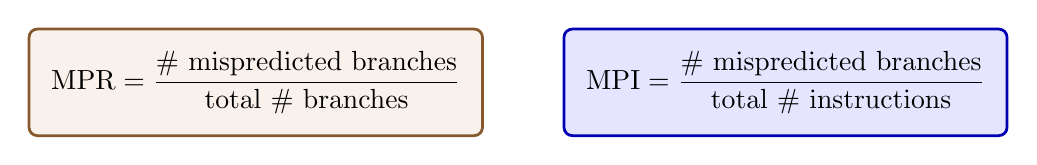
\begin{tikzpicture}
    % MPR box
    \node[draw=brown!70!black, line width=1pt, fill=brown!10, rounded corners=3pt,
          inner sep=8pt, font=\normalsize] (mpr) at (0,0) {
        $\text{MPR} = \dfrac{\text{\# mispredicted branches}}{\text{total \# branches}}$
    };

    % MPI box
    \node[draw=blue!70!black, line width=1pt, fill=blue!10, rounded corners=3pt,
          inner sep=8pt, font=\normalsize, right=1cm of mpr] (mpi) {
        $\text{MPI} = \dfrac{\text{\# mispredicted branches}}{\text{total \# instructions}}$
    };
\end{tikzpicture}
\end{center}

\vspace{0.1cm}

\begin{itemize}
    \item \textcolor{blue!70!black}{\textbf{MPI}} correlates better with performance -- accounts for branch frequency
\end{itemize}

\vspace{0.2cm}

\begin{columns}[T]
\begin{column}{0.48\textwidth}
\begin{tcolorbox}[
    colback=lightgreen!15,
    colframe=mygreen!80!black,
    boxrule=1pt,
    arc=2mm,
    title={\textbf{Assume}},
    fonttitle=\small
]
\small
\begin{itemize}
    \item MPI = 1\%
    \item IPC = 2
    \item Flush penalty = 10 cycles
\end{itemize}
\end{tcolorbox}
\end{column}

\begin{column}{0.48\textwidth}
\begin{tcolorbox}[
    colback=myorange!10,
    colframe=myorange!80!black,
    boxrule=1pt,
    arc=2mm,
    title={\textbf{Result}},
    fonttitle=\small
]
\small
\begin{itemize}
    \item 1 flush / 100 instructions
    \item $\Rightarrow$ 1 flush / 50 cycles
    \item $\Rightarrow$ \textbf{\textcolor{red!70!black}{20\% performance loss!}}
\end{itemize}
\end{tcolorbox}
\end{column}
\end{columns}

\end{frame}

\begin{frame}
\frametitle{What/Who/When We Predict/Fix/Allocate}
\label{frame:predict_fix_allocate}

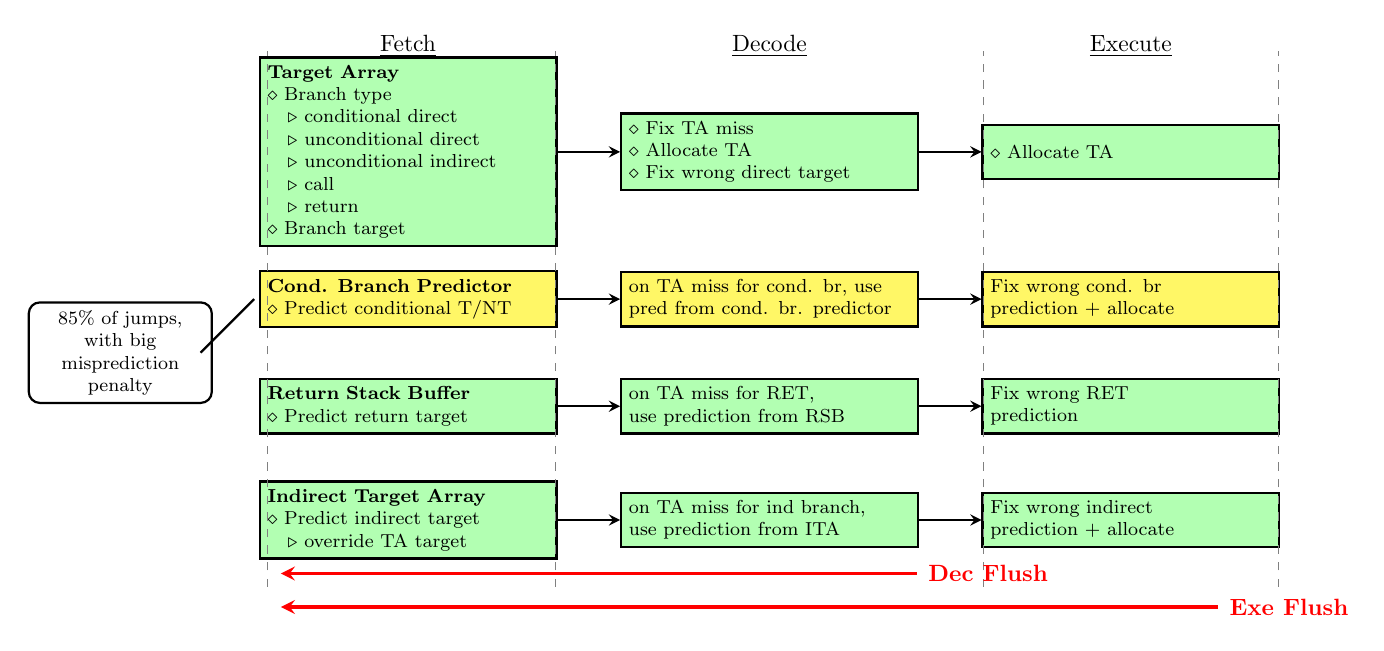
\begin{tikzpicture}[scale=0.85, transform shape,
    box/.style={rectangle, draw=black, thick, minimum height=0.8cm, text width=4.2cm, align=left, font=\footnotesize},
    greenbox/.style={box, fill=green!30},
    yellowbox/.style={box, fill=yellow!60},
    arrow/.style={->, thick, >=stealth}
]

% Column headers
\node[font=\normalsize, anchor=south] at (2.1, 5.8) {\underline{Fetch}};
\node[font=\normalsize, anchor=south] at (7.5, 5.8) {\underline{Decode}};
\node[font=\normalsize, anchor=south] at (12.9, 5.8) {\underline{Execute}};

% Fetch column
\node[greenbox] (ta) at (2.1, 4.5) {
    \textbf{Target Array}\\
    $\diamond$ Branch type\\
    \hspace{0.3cm}$\triangleright$ conditional direct\\
    \hspace{0.3cm}$\triangleright$ unconditional direct\\
    \hspace{0.3cm}$\triangleright$ unconditional indirect\\
    \hspace{0.3cm}$\triangleright$ call\\
    \hspace{0.3cm}$\triangleright$ return\\
    $\diamond$ Branch target
};

\node[yellowbox] (cbp) at (2.1, 2.3) {
    \textbf{Cond. Branch Predictor}\\
    $\diamond$ Predict conditional T/NT
};

\node[greenbox] (rsb) at (2.1, 0.7) {
    \textbf{Return Stack Buffer}\\
    $\diamond$ Predict return target
};

\node[greenbox] (ita) at (2.1, -1.0) {
    \textbf{Indirect Target Array}\\
    $\diamond$ Predict indirect target\\
    \hspace{0.3cm}$\triangleright$ override TA target
};

% Decode column
\node[greenbox] (dec1) at (7.5, 4.5) {
    $\diamond$ Fix TA miss\\
    $\diamond$ Allocate TA\\
    $\diamond$ Fix wrong direct target
};

\node[yellowbox] (dec2) at (7.5, 2.3) {
    on TA miss for cond. br, use\\
    pred from cond. br. predictor
};

\node[greenbox] (dec3) at (7.5, 0.7) {
    on TA miss for RET,\\
    use prediction from RSB
};

\node[greenbox] (dec4) at (7.5, -1.0) {
    on TA miss for ind branch,\\
    use prediction from ITA
};

% Execute column
\node[greenbox] (exe1) at (12.9, 4.5) {
    $\diamond$ Allocate TA
};

\node[yellowbox] (exe2) at (12.9, 2.3) {
    Fix wrong cond. br\\
    prediction + allocate
};

\node[greenbox] (exe3) at (12.9, 0.7) {
    Fix wrong RET\\
    prediction
};

\node[greenbox] (exe4) at (12.9, -1.0) {
    Fix wrong indirect\\
    prediction + allocate
};

% Arrows between columns
\draw[arrow] (ta.east) -- (dec1.west);
\draw[arrow] (cbp.east) -- (dec2.west);
\draw[arrow] (rsb.east) -- (dec3.west);
\draw[arrow] (ita.east) -- (dec4.west);

\draw[arrow] (dec1.east) -- (exe1.west);
\draw[arrow] (dec2.east) -- (exe2.west);
\draw[arrow] (dec3.east) -- (exe3.west);
\draw[arrow] (dec4.east) -- (exe4.west);

% Vertical dashed lines
\draw[dashed, gray] (0, -2) -- (0, 6);
\draw[dashed, gray] (4.3, -2) -- (4.3, 6);
\draw[dashed, gray] (10.7, -2) -- (10.7, 6);
\draw[dashed, gray] (15.1, -2) -- (15.1, 6);

% Left annotation
\node[draw, rounded corners, thick, text width=2.5cm, align=center, font=\footnotesize] at (-2.2, 1.5) {
    85\% of jumps,\\
    with big\\
    misprediction\\
    penalty
};
\draw[thick] (-1.0, 1.5) -- (-0.2, 2.3);


% Red flush arrows (arrow ends just before the text)
\draw[arrow, red, very thick] (9.7, -1.8) -- (0.2, -1.8);
\node[red, font=\normalsize, anchor=west] at (9.75, -1.8) {\textbf{Dec Flush}};

\draw[arrow, red, very thick] (14.2, -2.3) -- (0.2, -2.3);
\node[red, font=\normalsize, anchor=west] at (14.25, -2.3) {\textbf{Exe Flush}};

\end{tikzpicture}

\end{frame}

\section{The Target Array}

\begin{frame}
\frametitle{Target Array}
\label{frame:target_array}

\begin{columns}[T]
\begin{column}{0.58\textwidth}
\begin{itemize}
    \item \textbf{The TA is accessed using the branch address (branch IP)}
    \begin{itemize}
        \item Implemented as an $n$-way set associative cache
    \end{itemize}
\end{itemize}

\vspace{0.15cm}

\begin{itemize}
    \item \textbf{The TA predicts the following}
    \begin{itemize}
        \item Instruction is a branch
        \item Predicted target
        \item Branch type
        \begin{itemize}
            \item Conditional: jump to target if predict taken
            \item Unconditional direct: take target
            \item Unconditional Indirect: if ITA hits, use its target
            \item Return: get target from Return Stack Buffer
        \end{itemize}
    \end{itemize}
\end{itemize}

\vspace{0.15cm}

\begin{itemize}
    \item \textbf{The TA is allocated/updated at Decode / EXE}
\end{itemize}

\vspace{0.15cm}

\begin{itemize}
    \item \textbf{Tags are usually partial}
    \begin{itemize}
        \item Trade-off space, can get false hits
        \item Few branches aliased to same entry
        \item No \textit{correctness}, only \textit{performance}
    \end{itemize}
\end{itemize}
\end{column}

\begin{column}{0.42\textwidth}
\vspace{0.5cm}
\begin{center}
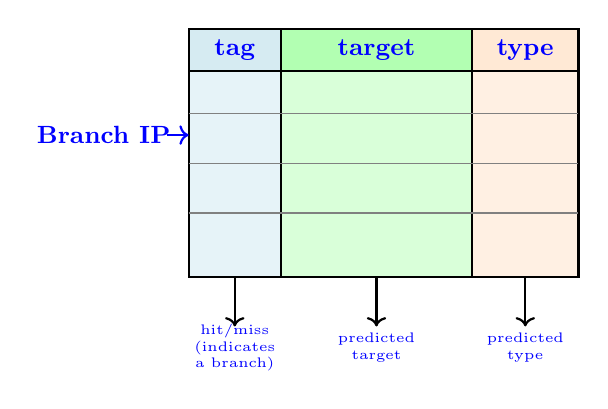
\begin{tikzpicture}[scale=0.9]
    % Define dimensions
    \def\tablewidth{5.5}
    \def\tableheight{3.5}
    \def\headerheight{0.6}
    \def\tagwidth{1.3}
    \def\targetwidth{2.7}
    \def\typewidth{1.5}
    
    % Draw the main table structure with colored columns
    % Tag column background
    \fill[lightblue!30] (0,0) rectangle (\tagwidth, -\tableheight);
    % Target column background  
    \fill[green!15] (\tagwidth,0) rectangle (\tagwidth+\targetwidth, -\tableheight);
    % Type column background
    \fill[peach!40] (\tagwidth+\targetwidth,0) rectangle (\tablewidth, -\tableheight);
    
    % Draw header row with stronger colors
    \fill[lightblue!50] (0,0) rectangle (\tagwidth, -\headerheight);
    \fill[green!30] (\tagwidth,0) rectangle (\tagwidth+\targetwidth, -\headerheight);
    \fill[peach!60] (\tagwidth+\targetwidth,0) rectangle (\tablewidth, -\headerheight);
    
    % Draw the table border
    \draw[thick, black] (0,0) rectangle (\tablewidth, -\tableheight);
    
    % Draw column dividers
    \draw[thick] (\tagwidth, 0) -- (\tagwidth, -\tableheight);
    \draw[thick] (\tagwidth+\targetwidth, 0) -- (\tagwidth+\targetwidth, -\tableheight);
    
    % Draw header separator
    \draw[thick] (0, -\headerheight) -- (\tablewidth, -\headerheight);
    
    % Add some row lines to show it's a table
    \foreach \y in {1.2, 1.9, 2.6} {
        \draw[gray, thin] (0, -\y) -- (\tablewidth, -\y);
    }
    
    % Header labels
    \node[myblue, font=\small\bfseries] at (\tagwidth/2, -\headerheight/2) {tag};
    \node[myblue, font=\small\bfseries] at (\tagwidth+\targetwidth/2, -\headerheight/2) {target};
    \node[myblue, font=\small\bfseries] at (\tagwidth+\targetwidth+\typewidth/2, -\headerheight/2) {type};
    
    % Branch IP label and arrow pointing to table
    \node[myblue, font=\small\bfseries] at (-1.2, -1.5) {Branch IP};
    \draw[->, thick, myblue] (-0.3, -1.5) -- (0, -1.5);
    
    % Output arrows and labels below the table
    \draw[->, thick] (\tagwidth/2, -\tableheight) -- (\tagwidth/2, -\tableheight-0.7);
    \node[align=center, font=\tiny, myblue] at (\tagwidth/2, -\tableheight-1.0) {hit/miss\\(indicates\\a branch)};
    
    \draw[->, thick] (\tagwidth+\targetwidth/2, -\tableheight) -- (\tagwidth+\targetwidth/2, -\tableheight-0.7);
    \node[align=center, font=\tiny, myblue] at (\tagwidth+\targetwidth/2, -\tableheight-1.0) {predicted\\target};
    
    \draw[->, thick] (\tagwidth+\targetwidth+\typewidth/2, -\tableheight) -- (\tagwidth+\targetwidth+\typewidth/2, -\tableheight-0.7);
    \node[align=center, font=\tiny, myblue] at (\tagwidth+\targetwidth+\typewidth/2, -\tableheight-1.0) {predicted\\type};
\end{tikzpicture}
\end{center}
\end{column}
\end{columns}

\end{frame}




\begin{frame}{The Target Array}
\begin{columns}[T,onlytextwidth]
  \begin{column}{0.63\textwidth}
    \begin{itemize}
      \item The TA is accessed using the branch address (branch IP)
      \begin{itemize}
        \item Implemented as an $n$-way set associative cache
      \end{itemize}

      \item The TA predicts the following
      \begin{itemize}
        \item Instruction is a branch
        \item Predicted target
        \item Branch type
        \begin{itemize}
          \item Conditional: jump to target if predict taken
          \item Unconditional direct: take target
          \item Unconditional indirect: if iTA hits, use its target
          \item Return: get target from Return Stack Buffer
        \end{itemize}
      \end{itemize}

      \item The TA is allocated/updated at Decode / EXE

      \item Tags are usually partial
      \begin{itemize}
        \item Trade-off space, can get false hits
        \item Few branches aliased to same entry
        \item No correctness, only performance
      \end{itemize}
    \end{itemize}
  \end{column}

  \begin{column}{0.37\textwidth}
    \centering
    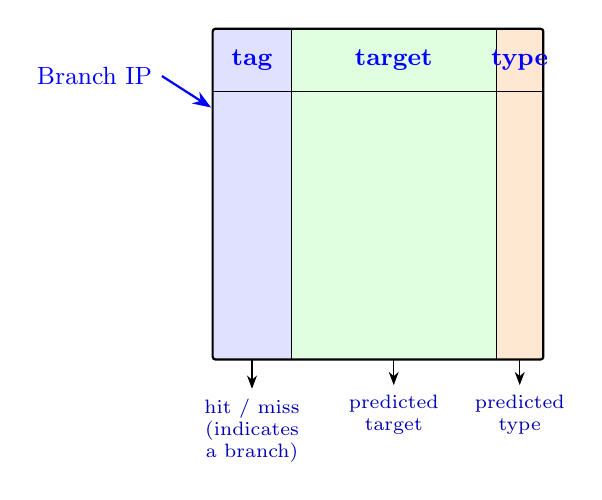
\begin{tikzpicture}[>=Stealth, node distance=2mm]
      % Sizes
      \def\W{4.2}   % total width
      \def\H{4.2}   % total height
      \def\tagw{1.0}
      \def\targetw{2.6}
      \def\typew{0.6}

      % Background column tints
      \fill[blue!12]   (0,-\H) rectangle (\tagw,0);
      \fill[green!12]  (\tagw,-\H) rectangle (\tagw+\targetw,0);
      \fill[orange!18] (\tagw+\targetw,-\H) rectangle (\W,0);

      % Outer box
      \draw[rounded corners=1pt, line width=0.8pt] (0,0) rectangle (\W,-\H);

      % Column dividers
      \draw (\tagw,0) -- (\tagw,-\H);
      \draw (\tagw+\targetw,0) -- (\tagw+\targetw,-\H);

      % Header separator
      \draw (0,-0.8) -- (\W,-0.8);

      % Header labels
      \node[font=\small\bfseries,blue]   at ($(0,0)!0.5!(\tagw,0)+(0,-0.4)$) {tag};
      \node[font=\small\bfseries,blue]   at ($(\tagw,0)!0.5!(\tagw+\targetw,0)+(0,-0.4)$) {target};
      \node[font=\small\bfseries,blue]   at ($(\tagw+\targetw,0)!0.5!(\W,0)+(0,-0.4)$) {type};

      % Branch IP input (left)
      \node[align=left, blue] (bp) at (-1.5,-0.6) {\small Branch IP};
      \draw[->,blue,thick] (bp.east) -- (-0.02,-1.0);

      % Bottom outputs
      \node[align=center, font=\scriptsize, blue!70!black] (hit) at (\tagw/2,-\H-0.9) {hit / miss\\(indicates\\a branch)};
      \draw[->] (\tagw/2,-\H) -- (hit.north);

      \node[align=center, font=\scriptsize, blue!70!black] (pt) at (\tagw+\targetw/2,-\H-0.7) {predicted\\target};
      \draw[->] (\tagw+\targetw/2,-\H) -- (pt.north);

      \node[align=center, font=\scriptsize, blue!70!black] (ty) at (\tagw+\targetw+\typew/2,-\H-0.7) {predicted\\type};
      \draw[->] (\tagw+\targetw+\typew/2,-\H) -- (ty.north);
    \end{tikzpicture}
  \end{column}
\end{columns}
\end{frame}

\section{Conditional Branch Direction Prediction}

% Section title - Conditional Branch Direction Prediction
\begin{frame}
\begin{center}
\vspace{2cm}
{\Huge\textcolor{myblue}{\textbf{Conditional Branch}}}

\vspace{0.3cm}

{\Huge\textcolor{myblue}{\textbf{Direction Prediction}}}
\end{center}
\end{frame}

% One-Bit Predictor
\begin{frame}
\frametitle{One-Bit Predictor}
\label{frame:one_bit_predictor}

\begin{center}
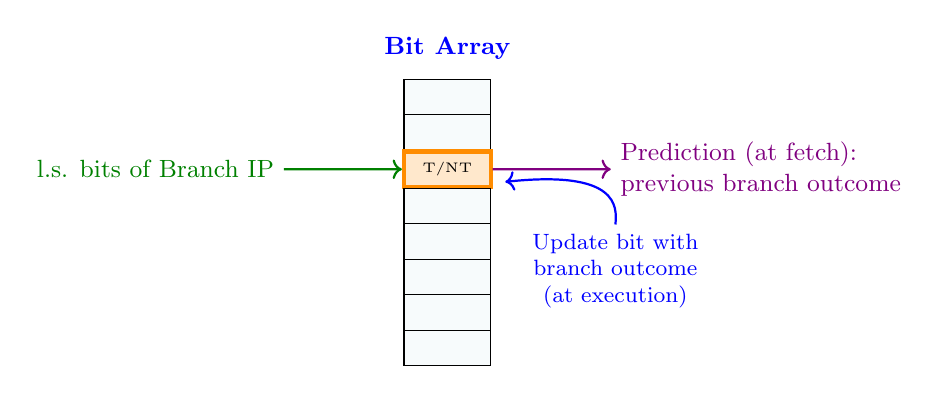
\begin{tikzpicture}[scale=0.8]
    % Bit array as matrix of nodes
    \matrix[matrix of nodes,
            nodes={draw, minimum width=1.1cm, minimum height=0.45cm, anchor=center, fill=lightblue!10, inner sep=1pt},
            row sep=-\pgflinewidth, column sep=-\pgflinewidth] (bit_array) {
        |[fill=lightblue!10]| \\
        |[fill=lightblue!10]| \\
        |[draw=myorange, line width=1.5pt, fill=myorange!20, font=\tiny]| T/NT \\
        |[fill=lightblue!10]| \\
        |[fill=lightblue!10]| \\
        |[fill=lightblue!10]| \\
        |[fill=lightblue!10]| \\
        |[fill=lightblue!10]| \\
    };
    \node[anchor=south,font=\small\bfseries,myblue] at (bit_array.north) {Bit Array};

    % Input label - positioned relative to highlighted cell
    \node[mygreen,anchor=east,font=\small,left=1.5cm of bit_array-3-1.west] (ls_bits) {l.s. bits of Branch IP};
    \draw[->,thick,mygreen] (ls_bits.east) -- (bit_array-3-1.west);

    % Output label - positioned relative to highlighted cell
    \node[mypurple,anchor=west,font=\small,align=left,right=1.5cm of bit_array-3-1.east] (prediction) {Prediction (at fetch):\\previous branch outcome};
    \draw[->,thick,mypurple] (bit_array-3-1.east) -- (prediction.west);

    % Curved arrow for update - relative positioning
    \node[myblue,align=center,anchor=north west,font=\footnotesize] at ([xshift=5mm]bit_array-4-1.south east) (update) {Update bit with\\branch outcome\\(at execution)};
    \draw[->,thick,myblue] (update.north) .. controls ([xshift=2cm]bit_array-4-1.east) and ([xshift=2cm]bit_array-3-1.east) .. ([xshift=2mm,yshift=-2mm]bit_array-3-1.east);
\end{tikzpicture}
\end{center}

\vspace{0.3cm}

\begin{itemize}
    \item \textbf{Problem: 1-bit predictor has a double mistake in loops}
\end{itemize}

\vspace{0.1cm}

{\footnotesize
\begin{tabular}{@{}ll@{}}
Branch Outcome & \texttt{0 0 0 0 0 1 0 0 0 0 0 1 0 0 0 0 0 1} \\
Prediction & \texttt{?~0 0 0 0 \textcolor{red}{0 1} 0 0 0 0 \textcolor{red}{0 1} 0 0 0 0 0} \\
\end{tabular}
}

\end{frame}

\subsection{Bimodal Predictors}

\begin{frame}
\frametitle{Bimodal (2-Bit) Predictor}
\label{frame:bimodal_2bit}

%\vspace{-0.3cm}

\begin{itemize}
    \item \textbf{2-bit counter:} needs ``more evidence'' to change prediction
\end{itemize}

\vspace{-0.2cm}

\begin{center}
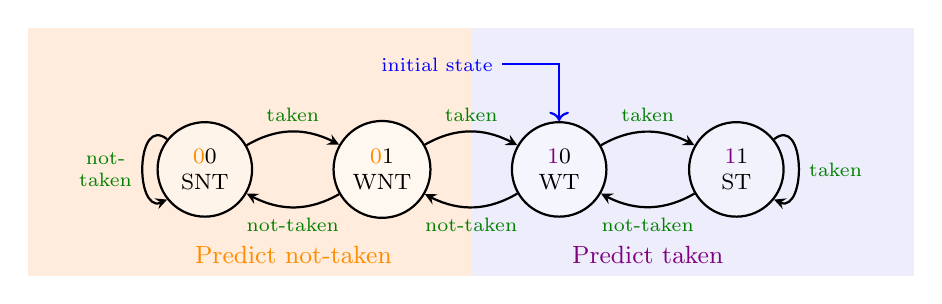
\begin{tikzpicture}[
    state/.style={circle,draw,thick,minimum size=1.2cm,font=\footnotesize,align=center},
    arrow/.style={->,>=stealth,thick},
    scale=0.9
]
    % Distinct background shades for prediction regions
    \begin{scope}[on background layer]
        \fill[peach!50] (-2.5,-1.5) rectangle (3.75,2); % Predict not-taken region
        \fill[lightpurple!70] (3.75,-1.5) rectangle (10,2); % Predict taken region, extended further right
    \end{scope}
    
    % States (LSB in black)
    \node[state,fill=peach!30] (SNT) at (0,0) {\textcolor{myorange}{0}\textcolor{black}{0}\\SNT};
    \node[state,fill=peach!20] (WNT) at (2.5,0) {\textcolor{myorange}{0}\textcolor{black}{1}\\WNT};
    \node[state,fill=lightpurple!40] (WT) at (5,0) {\textcolor{mypurple}{1}\textcolor{black}{0}\\WT};
    \node[state,fill=lightpurple!50] (ST) at (7.5,0) {\textcolor{mypurple}{1}\textcolor{black}{1}\\ST};
    
    % Self loop for SNT: from top left to bottom left, label on two lines
    \draw[arrow] (SNT) .. controls (-1,0.8) and (-1,-0.8) .. node[left,mygreen,font=\scriptsize,align=center] {not-\\taken} (SNT);
    % Self loop for ST: from top right to bottom right
    \draw[arrow] (ST) .. controls (8.5,0.8) and (8.5,-0.8) .. node[right,mygreen,font=\scriptsize,align=center] {taken} (ST);
    
    % Transitions between states
    \draw[arrow] (SNT) to[bend left=30] node[above,mygreen,font=\scriptsize] {taken} (WNT);
    \draw[arrow] (WNT) to[bend left=30] node[below,mygreen,font=\scriptsize] {not-taken} (SNT);
    
    \draw[arrow] (WNT) to[bend left=30] node[above,mygreen,font=\scriptsize] {taken} (WT);
    \draw[arrow] (WT) to[bend left=30] node[below,mygreen,font=\scriptsize] {not-taken} (WNT);
    
    \draw[arrow] (WT) to[bend left=30] node[above,mygreen,font=\scriptsize] {taken} (ST);
    \draw[arrow] (ST) to[bend left=30] node[below,mygreen,font=\scriptsize] {not-taken} (WT);
    
    % Prediction labels
    \node[myorange,font=\small] at (1.25,-1.2) {Predict not-taken};
    \node[mypurple,font=\small] at (6.25,-1.2) {Predict taken};

    % Initial state indicator
    \node[myblue,font=\scriptsize,anchor=east] (initial) at ([xshift=-0.8cm,yshift=0.8cm]WT.north) {initial state};
    \draw[->,thick,myblue] (initial.east) -| (WT.north);
\end{tikzpicture}
\end{center}

\vspace{0.1cm}

\begin{itemize}
    \item \textbf{Initial state:} weakly-taken (most branches are taken)
    \item \textbf{Update (at execution):}
    \begin{itemize}
        \item Taken $\rightarrow$ increment (saturate at 11); Not-taken $\rightarrow$ decrement (saturate at 00)
    \end{itemize}
    \item \textbf{Prediction:} m.s.bit of counter (0=NT, 1=T)
    \item Does not predict well patterns like 010101...
\end{itemize}

\end{frame}

\begin{frame}[fragile]
\frametitle{Bimodal Predictor Example}
\label{frame:bimodal_example}

\begin{columns}[T]
\begin{column}{0.45\textwidth}

{\small
\underline{\textbf{Br1 prediction}}
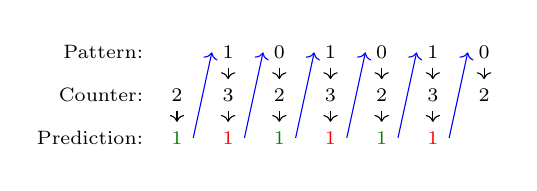
\begin{tikzpicture}[baseline=(current bounding box.center),every node/.style={anchor=base,font=\scriptsize}]
    \matrix[matrix of nodes,nodes={minimum width=0.4cm,anchor=center},column sep=0.25cm,row sep=0.15cm,ampersand replacement=\&] (m) {
        \phantom{0} \& 1 \& 0 \& 1 \& 0 \& 1 \& 0 \\
        2 \& 3 \& 2 \& 3 \& 2 \& 3 \& 2 \\
        \textcolor{mygreen}{1} \& \textcolor{red}{1} \& \textcolor{mygreen}{1} \& \textcolor{red}{1} \& \textcolor{mygreen}{1} \& \textcolor{red}{1} \& \phantom{0} \\
    };
    \foreach \i in {2,...,7} {
        \draw[->,thin] (m-1-\i.south) -- (m-2-\i.north);
    }
    \foreach \i in {1,...,6} {
        \draw[->,thin] (m-2-\i.south) -- (m-3-\i.north);
    }
    \foreach \i in {1,...,6} {
        \pgfmathtruncatemacro{\j}{\i+1}
        \draw[->,thin,myblue] (m-3-\i.east) -- (m-1-\j.west);
    }
    \node[left=0.1cm of m-1-1,align=right,font=\scriptsize] {Pattern:};
    \node[left=0.1cm of m-2-1,align=right,font=\scriptsize] {Counter:};
    \node[left=0.1cm of m-3-1,align=right,font=\scriptsize] {Prediction:};
\end{tikzpicture}

\vspace{0.1cm}
\underline{\textbf{Br2 prediction}}
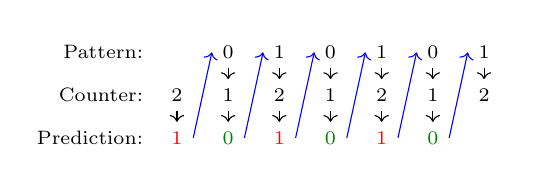
\begin{tikzpicture}[baseline=(current bounding box.center),every node/.style={anchor=base,font=\scriptsize}]
    \matrix[matrix of nodes,nodes={minimum width=0.4cm,anchor=center},column sep=0.25cm,row sep=0.15cm,ampersand replacement=\&] (m) {
        \phantom{0} \& 0 \& 1 \& 0 \& 1 \& 0 \& 1 \\
        2 \& 1 \& 2 \& 1 \& 2 \& 1 \& 2 \\
        \textcolor{red}{1} \& \textcolor{mygreen}{0} \& \textcolor{red}{1} \& \textcolor{mygreen}{0} \& \textcolor{red}{1} \& \textcolor{mygreen}{0} \& \phantom{0} \\
    };
    \foreach \i in {2,...,7} {
        \draw[->,thin] (m-1-\i.south) -- (m-2-\i.north);
    }
    \foreach \i in {1,...,6} {
        \draw[->,thin] (m-2-\i.south) -- (m-3-\i.north);
    }
    \foreach \i in {1,...,6} {
        \pgfmathtruncatemacro{\j}{\i+1}
        \draw[->,thin,myblue] (m-3-\i.east) -- (m-1-\j.west);
    }
    \node[left=0.1cm of m-1-1,align=right,font=\scriptsize] {Pattern:};
    \node[left=0.1cm of m-2-1,align=right,font=\scriptsize] {Counter:};
    \node[left=0.1cm of m-3-1,align=right,font=\scriptsize] {Prediction:};
\end{tikzpicture}

\vspace{0.1cm}
\underline{\textbf{Br3 prediction}}
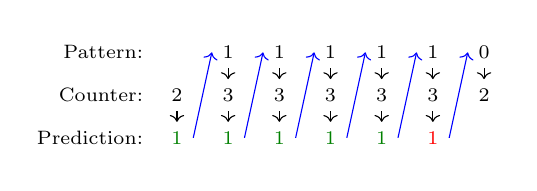
\begin{tikzpicture}[baseline=(current bounding box.center),every node/.style={anchor=base,font=\scriptsize}]
    \matrix[matrix of nodes,nodes={minimum width=0.4cm,anchor=center},column sep=0.25cm,row sep=0.15cm,ampersand replacement=\&] (m) {
        \phantom{0} \& 1 \& 1 \& 1 \& 1 \& 1 \& 0 \\
        2 \& 3 \& 3 \& 3 \& 3 \& 3 \& 2 \\
        \textcolor{mygreen}{1} \& \textcolor{mygreen}{1} \& \textcolor{mygreen}{1} \& \textcolor{mygreen}{1} \& \textcolor{mygreen}{1} \& \textcolor{red}{1} \& \phantom{0} \\
    };
    \foreach \i in {2,...,7} {
        \draw[->,thin] (m-1-\i.south) -- (m-2-\i.north);
    }
    \foreach \i in {1,...,6} {
        \draw[->,thin] (m-2-\i.south) -- (m-3-\i.north);
    }
    \foreach \i in {1,...,6} {
        \pgfmathtruncatemacro{\j}{\i+1}
        \draw[->,thin,myblue] (m-3-\i.east) -- (m-1-\j.west);
    }
    \node[left=0.1cm of m-1-1,align=right,font=\scriptsize] {Pattern:};
    \node[left=0.1cm of m-2-1,align=right,font=\scriptsize] {Counter:};
    \node[left=0.1cm of m-3-1,align=right,font=\scriptsize] {Prediction:};
\end{tikzpicture}
}

\end{column}

\begin{column}{0.55\textwidth}
\vspace{0.5cm}
\textbf{\small Code:}
\vspace{0.1cm}

\begin{tcolorbox}[
    colback=lightblue!10,
    colframe=myblue,
    boxrule=1pt,
    arc=2mm,
    left=1mm,
    right=1mm,
    top=1mm,
    bottom=1mm
]
\begin{lstlisting}[basicstyle=\footnotesize\ttfamily]
int n = 6;
do {
  ...
  if (n % 2) {...}     // br1
  if ((n+1) % 2) {...} // br2
} while (--n);         // br3
\end{lstlisting}
\end{tcolorbox}
\end{column}
\end{columns}

\end{frame}

\subsection{2-Level Branch Prediction}

\begin{frame}[t]
\frametitle{2-Level Branch Prediction}
\label{frame:2level_prediction}

\begin{columns}[T]
\begin{column}{0.72\textwidth}
\begin{itemize}
    \item Save branch direction history in a Branch History Register (BHR)
    \begin{itemize}
        \item A shift-register that saves the last $n$ outcomes
        \item History points to Pattern History Table ($2^n$ entries)
        \item PHT entry specifies predicted direction for that history
    \end{itemize}
    \item Example: pattern 0001 0001 ... with $n=3$
\end{itemize}
\end{column}
\begin{column}{0.28\textwidth}
\end{column}
\end{columns}

\vspace{-0.3cm}

\begin{tikzpicture}[remember picture,overlay,
    every node/.style={font=\small},
    bhr/.style={draw,thick,fill=lightgreen!50,minimum width=0.5cm,minimum height=0.5cm},
    actual/.style={draw,thick,fill=yellow!50,minimum width=0.5cm,minimum height=0.5cm},
    other/.style={draw,thin,gray!50,text=gray,minimum width=0.5cm,minimum height=0.5cm}
]
    % PHT on the right (overlay)
    \matrix[matrix of nodes,
        nodes={draw,thick,fill=lightblue!20,minimum width=0.55cm,minimum height=0.4cm,anchor=center,font=\scriptsize},
        row sep=0cm,ampersand replacement=\&,
        anchor=north east,
        at={($(current page.north east)+(-0.8cm,-2.2cm)$)}
    ] (pht) {
        |[alt=<2->{fill=myorange!40}{}]| \only<1>{?}\only<2->{\textbf{1}} \& |[draw=none,font=\tiny]| 000 \\
        |[alt=<3->{fill=myorange!40}{}]| \only<1-2>{?}\only<3->{\textbf{0}} \& |[draw=none,font=\tiny]| 001 \\
        |[alt=<4->{fill=myorange!40}{}]| \only<1-3>{?}\only<4->{\textbf{0}} \& |[draw=none,font=\tiny]| 010 \\
        ? \& |[draw=none,font=\tiny]| 011 \\
        |[alt=<5->{fill=myorange!40}{}]| \only<1-4>{?}\only<5->{\textbf{0}} \& |[draw=none,font=\tiny]| 100 \\
        ? \& |[draw=none,font=\tiny]| 101 \\
        ? \& |[draw=none,font=\tiny]| 110 \\
        ? \& |[draw=none,font=\tiny]| 111 \\
    };
    \node[above=0.1cm of pht-1-1,font=\footnotesize\bfseries] {PHT};

    % Branch outcomes sequence - positioned near bottom
    \matrix[matrix of nodes,nodes={minimum width=0.5cm,minimum height=0.5cm,anchor=center},column sep=0.08cm,ampersand replacement=\&,
        at={($(current page.south)+(0cm,2.8cm)$)}
    ] (seq) {
        |[alt=<1>{bhr}{other}]| 0 \&
        |[alt=<1-2>{bhr}{other}]| 0 \&
        |[alt=<1-3>{bhr}{other}]| 0 \&
        |[alt=<1>{actual}{alt=<2-4>{bhr}{other}}]| 1 \&
        |[alt=<2>{actual}{alt=<3-5>{bhr}{other}}]| 0 \&
        |[alt=<3>{actual}{alt=<4-6>{bhr}{other}}]| 0 \&
        |[alt=<4>{actual}{alt=<5-7>{bhr}{other}}]| 0 \&
        |[alt=<5>{actual}{alt=<6-8>{bhr}{other}}]| 1 \&
        |[alt=<6>{actual}{alt=<7-8>{bhr}{other}}]| 0 \&
        |[alt=<7>{actual}{alt=<8>{bhr}{other}}]| 0 \&
        |[alt=<8>{actual}{other}]| 0 \&
        |[other]| 1 \&
        |[draw=none,text=gray]| \ldots \\
    };

    % BHR box - shifts each stage
    \only<1>{\node[draw,very thick,rounded corners=2pt,fit=(seq-1-1)(seq-1-3),inner sep=1pt,label={[font=\footnotesize\bfseries]above:BHR}] (bhrbox) {};}
    \only<2>{\node[draw,very thick,rounded corners=2pt,fit=(seq-1-2)(seq-1-4),inner sep=1pt,label={[font=\footnotesize\bfseries]above:BHR}] (bhrbox) {};}
    \only<3>{\node[draw,very thick,rounded corners=2pt,fit=(seq-1-3)(seq-1-5),inner sep=1pt,label={[font=\footnotesize\bfseries]above:BHR}] (bhrbox) {};}
    \only<4>{\node[draw,very thick,rounded corners=2pt,fit=(seq-1-4)(seq-1-6),inner sep=1pt,label={[font=\footnotesize\bfseries]above:BHR}] (bhrbox) {};}
    \only<5>{\node[draw,very thick,rounded corners=2pt,fit=(seq-1-5)(seq-1-7),inner sep=1pt,label={[font=\footnotesize\bfseries]above:BHR}] (bhrbox) {};}
    \only<6>{\node[draw,very thick,rounded corners=2pt,fit=(seq-1-6)(seq-1-8),inner sep=1pt,label={[font=\footnotesize\bfseries]above:BHR}] (bhrbox) {};}
    \only<7>{\node[draw,very thick,rounded corners=2pt,fit=(seq-1-7)(seq-1-9),inner sep=1pt,label={[font=\footnotesize\bfseries]above:BHR}] (bhrbox) {};}
    \only<8>{\node[draw,very thick,rounded corners=2pt,fit=(seq-1-8)(seq-1-10),inner sep=1pt,label={[font=\footnotesize\bfseries]above:BHR}] (bhrbox) {};}

    % Arrows from BHR to actual PHT entries - smooth curve through high point
    \only<1>{\draw[->,thick] (bhrbox.north east) .. controls ++(6cm,1cm) and ++(-2cm,0) .. (pht-1-1.west);}
    \only<2>{\draw[->,thick] (bhrbox.north east) .. controls ++(4.7cm,0.7cm) and ++(-2cm,0) .. (pht-2-1.west);}
    \only<3>{\draw[->,thick] (bhrbox.north east) .. controls ++(4.4cm,0.4cm) and ++(-2cm,0) .. (pht-3-1.west);}
    \only<4>{\draw[->,thick] (bhrbox.north east) .. controls ++(4.1cm,1cm) and ++(-2cm,0) .. (pht-5-1.west);}
    \only<5>{\draw[->,thick] (bhrbox.north east) .. controls ++(3.8cm,1.3cm) and ++(-2cm,0) .. (pht-1-1.west);}
    \only<6>{\draw[->,thick] (bhrbox.north east) .. controls ++(3.5cm,1cm) and ++(-2cm,0) .. (pht-2-1.west);}
    \only<7>{\draw[->,thick] (bhrbox.north east) .. controls ++(3.2cm,0.7cm) and ++(-2cm,0) .. (pht-3-1.west);}
    \only<8>{\draw[->,thick] (bhrbox.north east) .. controls ++(2.9cm,1.3cm) and ++(-2cm,0) .. (pht-5-1.west);}

    % Checkmarks below yellow cell when prediction is correct (stages 5-8)
    \only<5>{\node[below=0.1cm of seq-1-8,mygreen,font=\small] {\checkmark};}
    \only<6>{\node[below=0.1cm of seq-1-9,mygreen,font=\small] {\checkmark};}
    \only<7>{\node[below=0.1cm of seq-1-10,mygreen,font=\small] {\checkmark};}
    \only<8>{\node[below=0.1cm of seq-1-11,mygreen,font=\small] {\checkmark};}

    % Labels
    \node[left=0.2cm of seq-1-1,font=\footnotesize] {Branches:};

    % Stage explanation in a box
    \node[below=0.7cm of seq,draw,fill=lightblue!15,rounded corners=3pt,inner sep=6pt,font=\footnotesize,align=left] {
        \only<1>{BHR=000 $\rightarrow$ predict PHT[000]=? $\rightarrow$ actual is \textbf{1} $\rightarrow$ update PHT[000]$\leftarrow$1}
        \only<2>{BHR=001 $\rightarrow$ predict PHT[001]=? $\rightarrow$ actual is \textbf{0} $\rightarrow$ update PHT[001]$\leftarrow$0}
        \only<3>{BHR=010 $\rightarrow$ predict PHT[010]=? $\rightarrow$ actual is \textbf{0} $\rightarrow$ update PHT[010]$\leftarrow$0}
        \only<4>{BHR=100 $\rightarrow$ predict PHT[100]=? $\rightarrow$ actual is \textbf{0} $\rightarrow$ update PHT[100]$\leftarrow$0}
        \only<5>{BHR=000 $\rightarrow$ predict PHT[000]=1 $\rightarrow$ actual is \textbf{1} \checkmark correct!}
        \only<6>{BHR=001 $\rightarrow$ predict PHT[001]=0 $\rightarrow$ actual is \textbf{0} \checkmark correct!}
        \only<7>{BHR=010 $\rightarrow$ predict PHT[010]=0 $\rightarrow$ actual is \textbf{0} \checkmark correct!}
        \only<8>{BHR=100 $\rightarrow$ predict PHT[100]=0 $\rightarrow$ actual is \textbf{0} \checkmark steady state}
    };
\end{tikzpicture}

\end{frame}

% Shortest History To Predict a Pattern
\begin{frame}[t]
\frametitle{Shortest History To Predict a Pattern}
\label{frame:shortest_history}

% Reduce colorbox padding
\setlength{\fboxsep}{1pt}

\begin{itemize}
    \item What is the shortest history needed to perfectly predict \texttt{10011 10011 ...} in steady state?
\end{itemize}

% History length 3
\begin{columns}[T]
\begin{column}{0.55\textwidth}
\begin{itemize}
    \item History of length 3 predicts correctly:
    \begin{itemize}
        \item \texttt{\colorbox{lightblue!30}{100}11 10011} \hspace{0.2cm} 100 $\Rightarrow$ 1
        \item \texttt{1\colorbox{lightblue!30}{001}1 10011} \hspace{0.2cm} 001 $\Rightarrow$ 1
        \item \texttt{10\colorbox{lightblue!30}{011} 10011} \hspace{0.2cm} 011 $\Rightarrow$ 1
        \item \texttt{100\colorbox{lightblue!30}{11 1}0011} \hspace{0.2cm} 111 $\Rightarrow$ 0
        \item \texttt{1001\colorbox{lightblue!30}{1 10}011} \hspace{0.2cm} 110 $\Rightarrow$ 0
    \end{itemize}
\end{itemize}
\end{column}
\begin{column}{0.42\textwidth}
\vspace{0.5cm}
\begin{tcolorbox}[colback=lightgreen!20,colframe=mygreen,boxrule=0.5pt,arc=2pt,left=3pt,right=3pt,top=2pt,bottom=2pt]
\small No sub-pattern appears more than once, or it always points to the same value
\end{tcolorbox}
\end{column}
\end{columns}

\vspace{0.2cm}

% History length 2
\begin{columns}[T]
\begin{column}{0.55\textwidth}
\begin{itemize}
    \item History of length 2 is wrong twice:
    \begin{itemize}
        \item \texttt{\colorbox{lightblue!30}{10}011 10011} \hspace{0.2cm} 10 $\Rightarrow$ 0
        \item \texttt{1\colorbox{lightblue!30}{00}11 10011} \hspace{0.2cm} 00 $\Rightarrow$ 1
        \item \texttt{10\colorbox{lightblue!30}{01}1 10011} \hspace{0.2cm} 01 $\Rightarrow$ 1
        \item \texttt{100\colorbox{lightblue!30}{11} 10011} \hspace{0.2cm} 11 $\Rightarrow$ \textcolor{red}{1}
        \item \texttt{1001\colorbox{lightblue!30}{1 1}0011} \hspace{0.2cm} 11 $\Rightarrow$ \textcolor{red}{0}
    \end{itemize}
\end{itemize}
\end{column}
\begin{column}{0.42\textwidth}
\vspace{0.5cm}
\begin{tcolorbox}[colback=red!10,colframe=red!70,boxrule=0.5pt,arc=2pt,left=3pt,right=3pt,top=2pt,bottom=2pt]
\small Sub-pattern \texttt{11} appears twice, pointing to different values $\rightarrow$ conflict!
\end{tcolorbox}
\end{column}
\end{columns}

\end{frame}

\subsection{Local History Predictors}

\begin{frame}[t]
\frametitle{Local History Predictor}
\label{frame:local_history}

\begin{itemize}
    \item Use 2-bit saturating counters instead of 1 bit to record outcome
    \begin{itemize}
        \item Avoid double mistake when two history sub-patterns point to same value, or in case of a pattern \textcolor{red}{\textbf{glitch}}
        \item Example: \texttt{00001 00001 00001 0}\textcolor{red}{\textbf{1}}\texttt{001 00001 00001}
    \end{itemize}
\end{itemize}

\vspace{0.0cm}

\begin{center}
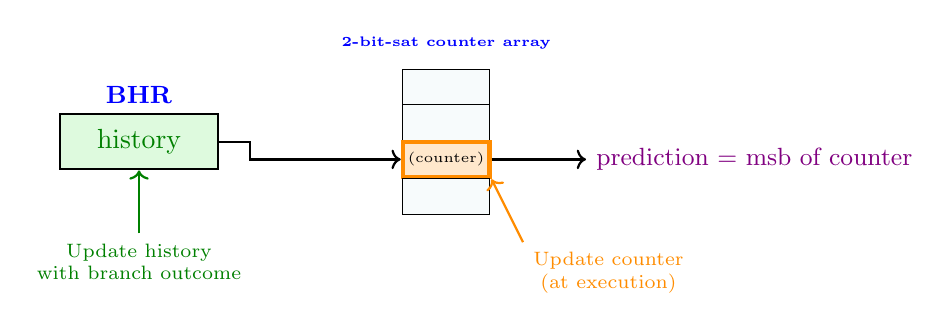
\begin{tikzpicture}[scale=0.8]
    % BHR
    \node[draw,thick,fill=lightgreen!30,minimum width=2cm,minimum height=0.7cm] (bhr) at (0,0) {\textcolor{mygreen}{history}};
    \node[anchor=south,font=\small\bfseries,myblue] at (bhr.north) {BHR};

    % Counter array as matrix of nodes
    \matrix[matrix of nodes,
            nodes={draw, minimum width=1.1cm, minimum height=0.45cm, anchor=center, fill=lightblue!10, inner sep=1pt},
            row sep=-\pgflinewidth, column sep=-\pgflinewidth,
            anchor=west] (counter_array) at (4,0) {
        |[fill=lightblue!10]| \\
        |[fill=lightblue!10]| \\
        |[draw=myorange, line width=1.5pt, fill=myorange!20, font=\tiny]| (counter) \\
        |[fill=lightblue!10]| \\
    };
    \node[anchor=south,font=\tiny\bfseries,myblue] at (counter_array.north) {2-bit-sat counter array};

    % Arrow from BHR to counter array
    \draw[->,thick] (bhr.east) -- ++(0.5,0) |- (counter_array-3-1.west);

    % Arrow from counter to prediction
    \draw[->,thick] (counter_array-3-1.east) -- ++(1.5,0)
        node[anchor=west,font=\small,mypurple] {prediction = msb of counter};

    % Update history arrow - points to BHR
    \draw[->,thick,mygreen] ($(bhr.south)+(0,-1)$) -- (bhr.south)
        node[pos=0,anchor=north,font=\scriptsize,align=center] {Update history\\with branch outcome};

    % Update counter arrow - points to the orange counter cell (row 3)
    \draw[->,thick,myorange] ($(counter_array-3-1.south east)+(0.5,-1)$) -- (counter_array-3-1.south east)
        node[pos=0,anchor=north west,font=\scriptsize,align=center] {Update counter\\(at execution)};
\end{tikzpicture}
\end{center}

\vspace{-0.2cm}

\begin{itemize}
    \item The longer the history:
    \begin{itemize}
        \item Warm-up is longer
        \item Counter array becomes very big (and sparse)
    \end{itemize}
\end{itemize}

\end{frame}

% Speculative History Updates - slide 1
\begin{frame}[t]
\frametitle{Speculative History Updates}
\label{frame:speculative_history_1}

\begin{itemize}
    \item Deep pipeline $\Rightarrow$ many cycles between fetch and branch resolution
    \begin{itemize}
        \item If history updated only at execution, future branches may use stale history
        \item Solution: update history speculatively according to prediction
    \end{itemize}
\end{itemize}

\vspace{0.2cm}

\begin{center}
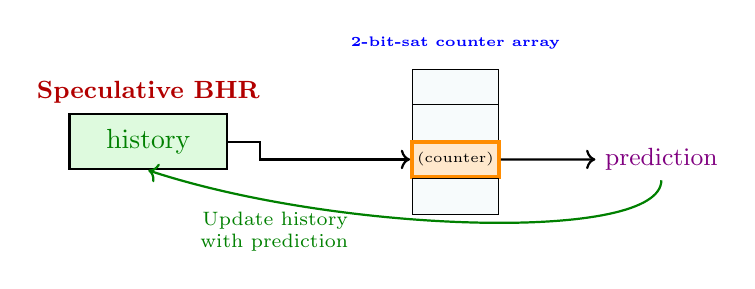
\begin{tikzpicture}[scale=0.8]
    % Speculative BHR
    \node[draw,thick,fill=lightgreen!30,minimum width=2cm,minimum height=0.7cm] (sbhr) at (0,0) {\textcolor{mygreen}{history}};
    \node[anchor=south,font=\small\bfseries,red!70!black] at (sbhr.north) {Speculative BHR};

    % Counter array as matrix of nodes
    \matrix[matrix of nodes,
            nodes={draw, minimum width=1.1cm, minimum height=0.45cm, anchor=center, fill=lightblue!10, inner sep=1pt},
            row sep=-\pgflinewidth, column sep=-\pgflinewidth,
            anchor=west] (counter_array) at (4,0) {
        |[fill=lightblue!10]| \\
        |[fill=lightblue!10]| \\
        |[draw=myorange, line width=1.5pt, fill=myorange!20, font=\tiny]| (counter) \\
        |[fill=lightblue!10]| \\
    };
    \node[anchor=south,font=\tiny\bfseries,myblue] at (counter_array.north) {2-bit-sat counter array};

    % Arrow from BHR to counter array
    \draw[->,thick] (sbhr.east) -- ++(0.5,0) |- (counter_array-3-1.west);

    % Arrow from counter to prediction
    \node[anchor=west,font=\small,mypurple] (pred) at ($(counter_array-3-1.east)+(1.5,0)$) {prediction};
    \draw[->,thick] (counter_array-3-1.east) -- (pred.west);

    % Speculative update: arrow from prediction back to history (from bottom)
    \draw[->,thick,mygreen] (pred.south) .. controls ++(0,-1) and ++(3,-1) .. (sbhr.south)
        node[pos=0.8,below,font=\scriptsize,align=right] {Update history\\with prediction};
\end{tikzpicture}
\end{center}

\vspace{0.2cm}

\begin{itemize}
    \item As long as predictions are correct, the history used for next branch is correct
\end{itemize}

\end{frame}

% Speculative History Updates - slide 2
\begin{frame}[t]
\frametitle{Speculative History: Misprediction Recovery}
\label{frame:speculative_history_2}

\begin{itemize}
    \item On misprediction: copy non-speculative BHR into speculative BHR
    \item Non-speculative BHR is updated at execution with actual branch outcome
\end{itemize}

\vspace{0.2cm}

\begin{center}
\begin{tikzpicture}[scale=0.8]
    % Counter array as matrix of nodes (center) - 4 entries for consistency
    \matrix[matrix of nodes,
            nodes={draw, minimum width=1.1cm, minimum height=0.45cm, anchor=center, fill=lightblue!10, inner sep=1pt},
            row sep=-\pgflinewidth, column sep=-\pgflinewidth] (counter_array) at (4,0) {
        |[fill=lightblue!10]| \\
        |[fill=lightblue!10]| \\
        |[draw=myorange, line width=1.5pt, fill=myorange!20, font=\tiny]| (counter) \\
        |[fill=lightblue!10]| \\
    };
    \node[anchor=south,font=\tiny\bfseries,myblue,align=center] at (counter_array.north) {2-bit-sat\\counter array};
    \node[anchor=north,font=\small] at (counter_array.south) {$\vdots$};

    % Speculative BHR (top left)
    \node[draw,thick,fill=lightgreen!30,minimum width=2.2cm,minimum height=0.7cm] (sbhr) at (0,1.2) {\textcolor{mygreen}{history}};
    \node[anchor=south,font=\small\bfseries,red!70!black] at (sbhr.north) {Speculative BHR};

    % BHR (bottom left)
    \node[draw,thick,fill=lightgreen!30,minimum width=2.2cm,minimum height=0.7cm] (bhr) at (0,-1.5) {\textcolor{mygreen}{history}};
    \node[anchor=south,font=\small\bfseries,myblue] at (bhr.north) {BHR};

    % Arrow from Speculative BHR to counter array
    \draw[->,thick,mygreen] (sbhr.east) -- ++(0.5,0) |- (counter_array-3-1.west);

    % Prediction output (more to the right)
    \node[anchor=west,font=\small,mypurple] (pred) at ($(counter_array-3-1.east)+(1.5,0)$) {prediction};
    \draw[->,thick] (counter_array-3-1.east) -- (pred.west);

    % Stage 1: At Fetch - arrow from prediction.north to sbhr.north east, more curvy
    \only<1->{
        \draw[->,thick,mygreen] (pred.north) .. controls ++(0,2.5) and ++(3,1) .. (sbhr.north east)
            node[pos=0.15,anchor=south west,font=\scriptsize,mygreen,align=left] {\textbf{At Fetch}:\\Update history\\with prediction};
    }

    % Stage 2: At Execution - arrow to update counter + BHR
    \only<2->{
        \node[anchor=north west,font=\scriptsize,myblue,align=left] (exec_label) at ($(counter_array-3-1.south east)+(0.5,-0.8)$) {\textbf{At Execution}:\\Update counter + BHR\\with branch outcome};
        \draw[->,thick,myblue] (exec_label.north west) -- (counter_array-3-1.south east);
        \draw[->,thick,myblue] (exec_label.west) .. controls ++(-1.5,0) and ++(1,0) .. (bhr.east);
    }

    % Stage 3: On Misprediction - curvy arrow from BHR.west to Speculative BHR.west
    \only<3->{
        \draw[->,thick,red,dashed] (bhr.west) .. controls ++(-1.5,0) and ++(-1.5,0) .. (sbhr.west)
            node[pos=0.5,anchor=east,font=\scriptsize,red,align=right,xshift=-2pt] {\textbf{On Misprediction}:\\copy to recover};
    }
\end{tikzpicture}
\end{center}

\end{frame}

% Speculative History Updates - slide 3
\begin{frame}[t]
\frametitle{Speculative History: Counter Array}
\label{frame:speculative_history_3}

\begin{itemize}
    \item The counter array is \textbf{not} updated speculatively
    \item Prediction changes only on misprediction (state $01\rightarrow10$ or $10\rightarrow01$)
    \item Counter array too big to recover after misprediction
    \begin{itemize}
        \item Too expensive to maintain both speculative and non-speculative copies
    \end{itemize}
\end{itemize}

\end{frame}

% Local Predictor: private counter arrays
\begin{frame}
\frametitle{Local Predictor: Private Counter Arrays}
\label{frame:local_private}

\textbf{Holding BHRs and counter arrays for many branches:}

\vspace{0.2cm}

\begin{center}
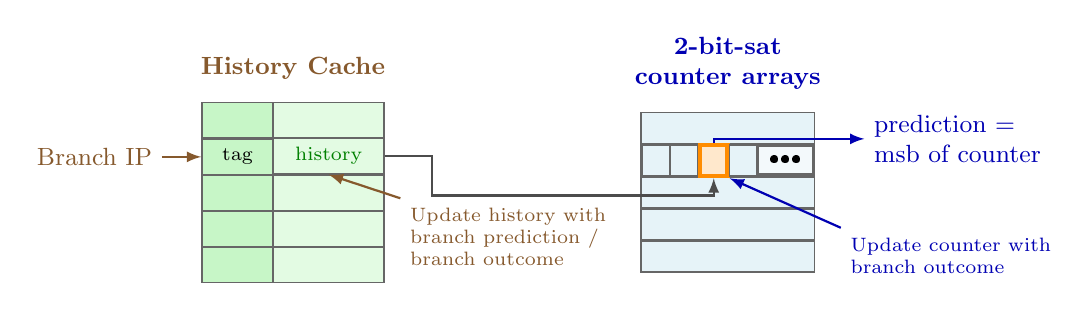
\begin{tikzpicture}[
    cache_cell/.style={draw=black!60, line width=0.6pt, minimum height=0.45cm, fill=lightgreen!30, inner sep=2pt, font=\scriptsize},
    counter_row/.style={draw=black!60, line width=0.6pt, minimum height=0.4cm, fill=lightblue!30, inner sep=1pt, font=\tiny},
    counter_cell/.style={draw=black!60, line width=0.6pt, minimum height=0.4cm, minimum width=0.35cm, fill=lightblue!30, inner sep=1pt, font=\tiny},
    arrow/.style={-latex, thick, draw=black!70}
]

    % History Cache using matrix of nodes
    \matrix[matrix of nodes,
        nodes={cache_cell},
        row sep=-\pgflinewidth,
        column sep=-\pgflinewidth,
        ampersand replacement=\&,
        label={[label distance=1pt]above:{\small\bfseries\color{brown!70!black}History Cache}}
    ] (hist_cache) {
        |[minimum width=0.9cm, fill=lightgreen!50]| \& |[minimum width=1.4cm, fill=lightgreen!25]| \\
        |[minimum width=0.9cm, fill=lightgreen!50]| tag \& |[minimum width=1.4cm, fill=lightgreen!25]| \textcolor{mygreen}{history} \\
        |[minimum width=0.9cm, fill=lightgreen!50]| \& |[minimum width=1.4cm, fill=lightgreen!25]| \\
        |[minimum width=0.9cm, fill=lightgreen!50]| \& |[minimum width=1.4cm, fill=lightgreen!25]| \\
        |[minimum width=0.9cm, fill=lightgreen!50]| \& |[minimum width=1.4cm, fill=lightgreen!25]| \\
    };

    % Branch IP input - positioned relative to tag cell
    \node[anchor=east, left=0.5cm of hist_cache-2-1.west, font=\small, text=brown!70!black] (ip) {Branch IP};
    \draw[arrow, brown!70!black] (ip.east) -- (hist_cache-2-1.west);

    % Counter arrays - table with multiple rows (single wide column each)
    \matrix[matrix of nodes,
        nodes={counter_row, minimum width=2.2cm},
        row sep=-\pgflinewidth,
        ampersand replacement=\&,
        right=3cm of hist_cache.east,
        anchor=west,
    ] (counter_table) {
        \phantom{x} \\
        \phantom{x} \\
        \phantom{x} \\
        \phantom{x} \\
        \phantom{x} \\
    };

    % Counter arrays title (separate node for two-line support)
    \node[above=1pt of counter_table.north, font=\small\bfseries, text=blue!70!black, align=center] {2-bit-sat\\counter arrays};

    % Overlay: multi-column cells on row 2
    \matrix[matrix of nodes,
        nodes={counter_cell},
        row sep=-\pgflinewidth,
        column sep=-\pgflinewidth,
        ampersand replacement=\&,
        at=(counter_table-2-1.center),
        anchor=center
    ] (counter_cells) {
        \phantom{} \& \phantom{} \& |[draw=myorange, line width=1.5pt, fill=myorange!20]| \phantom{} \& \phantom{} \& \phantom{} \& \phantom{} \\
    };

    % Dots on top of 4th cell with rectangle
    \node[draw=black!60, anchor=east, line width=0.6pt, fill=lightblue!15, minimum width=0.7cm, minimum height=0.35cm, font=\scriptsize]
        at (counter_cells-1-6.east) {\textbullet\textbullet\textbullet};

    % Arrow from history to counter arrays - nice path going right then down then -| to bottom of cell
    \draw[arrow] (hist_cache-2-2.east) -- ++(0.6,0) -- ++(0,-0.5) -| (counter_cells-1-3.south);

    % Prediction output
    \node[anchor=west, yshift=0.5cm, font=\small, text=blue!70!black, align=left] at ([xshift=5mm]counter_cells-1-3.south -| counter_table.east) (prediction) {prediction =\\msb of counter};

    % Arrow from counter to prediction
    \draw[arrow, blue!70!black] (counter_cells-1-3.north) |- (prediction.west);

    % Update history label - south east of history cell
    \node[anchor=north west, font=\scriptsize, text=brown!70!black, align=left] (update_hist) at ([xshift=0.2cm, yshift=-0.3cm]hist_cache-2-2.south east) {Update history with\\branch prediction /\\branch outcome};
    \draw[arrow, brown!70!black] (update_hist.north west) -- (hist_cache-2-2.south);

    % Update counter label - anchored south west relative to counter_table south east
    \node[anchor=south west, font=\scriptsize, text=blue!70!black, align=left] (update_counter) at ([xshift=0.2cm]counter_table.south east) {Update counter with\\branch outcome};
    \draw[arrow, blue!70!black] (update_counter.north west) -- (counter_cells-1-3.south east);

\end{tikzpicture}
\end{center}

\vspace{-0.2cm}

\begin{alertblock}{Local Predictor with Private Counters Size}
\small
Size = \#BHRs $\times$ (tag\_size + history\_size + 2 $\times$ $2^{\text{history\_size}}$)
\end{alertblock}

\textbf{Example:} \#BHRs = 1024; tag\_size=8; history\_size=6

$\Rightarrow$ size = 1024 $\times$ (8 + 6 + 2$\times 2^6$) = 142Kbit

\end{frame}

% Local Predictor: shared counter arrays
\begin{frame}
\frametitle{Local Predictor: Shared Counter Arrays}
\label{frame:local_shared}

\begin{itemize}
    \item \textbf{Single counter array shared by all BHRs} -- all histories index the same array
    \item Branches with similar patterns interfere with each other
    \item Interference can be constructive or destructive
\end{itemize}

\vspace{-0.2cm}

\begin{center}
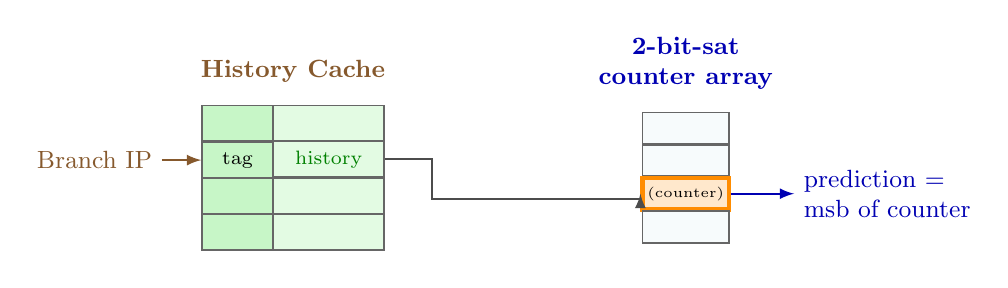
\begin{tikzpicture}[
    cache_cell/.style={draw=black!60, line width=0.6pt, minimum height=0.45cm, fill=lightgreen!30, inner sep=2pt, font=\scriptsize},
    counter_row/.style={draw=black!60, line width=0.6pt, minimum height=0.4cm, fill=lightblue!30, inner sep=1pt, font=\tiny},
    arrow/.style={-latex, thick, draw=black!70}
]

    % History Cache using matrix of nodes (4 rows)
    \matrix[matrix of nodes,
        nodes={cache_cell},
        row sep=-\pgflinewidth,
        column sep=-\pgflinewidth,
        ampersand replacement=\&,
        label={[label distance=1pt]above:{\small\bfseries\color{brown!70!black}History Cache}}
    ] (hist_cache) {
        |[minimum width=0.9cm, fill=lightgreen!50]| \& |[minimum width=1.4cm, fill=lightgreen!25]| \\
        |[minimum width=0.9cm, fill=lightgreen!50]| tag \& |[minimum width=1.4cm, fill=lightgreen!25]| \textcolor{mygreen}{history} \\
        |[minimum width=0.9cm, fill=lightgreen!50]| \& |[minimum width=1.4cm, fill=lightgreen!25]| \\
        |[minimum width=0.9cm, fill=lightgreen!50]| \& |[minimum width=1.4cm, fill=lightgreen!25]| \\
    };

    % Branch IP input - positioned relative to tag cell
    \node[anchor=east, left=0.5cm of hist_cache-2-1.west, font=\small, text=brown!70!black] (ip) {Branch IP};
    \draw[arrow, brown!70!black] (ip.east) -- (hist_cache-2-1.west);

    % Single shared counter array (vertical, 4 rows, highlight 3rd)
    \matrix[matrix of nodes,
        nodes={counter_row, minimum width=1.1cm},
        row sep=-\pgflinewidth,
        ampersand replacement=\&,
        right=3cm of hist_cache.east,
        anchor=west
    ] (counter_array) {
        |[fill=lightblue!10]| \\
        |[fill=lightblue!10]| \\
        |[draw=myorange, line width=1.5pt, fill=myorange!20, font=\tiny]| (counter) \\
        |[fill=lightblue!10]| \\
    };

    % Counter array title
    \node[above=1pt of counter_array.north, font=\small\bfseries, text=blue!70!black, align=center] {2-bit-sat\\counter array};

    % Arrow from history to counter array - nice path going right then down then -| to highlighted cell (row 3)
    \draw[arrow] (hist_cache-2-2.east) -- ++(0.6,0) -- ++(0,-0.5) -| (counter_array-3-1.west);

    % Prediction output - right of highlighted cell for straight arrow
    \node[anchor=west, right=0.8cm of counter_array-3-1.east, font=\small, text=blue!70!black, align=left] (prediction) {prediction =\\msb of counter};

    % Arrow from counter to prediction (straight)
    \draw[arrow, blue!70!black] (counter_array-3-1.east) -- (prediction.west);

\end{tikzpicture}
\end{center}

\vspace{-0.2cm}

\begin{alertblock}{Local Predictor with Shared Counter Size}
\small
Size = \#BHRs $\times$ (tag\_size + history\_size) + 2 $\times$ $2^{\text{history\_size}}$
\end{alertblock}

\textbf{Example:} \#BHRs = 1024; tag\_size=8; history\_size=6 $\Rightarrow$ size = 1024 $\times$ (8 + 6) + 2$\times 2^6$ = 14.1Kbit

\end{frame}

% Local Predictor: Lselect
\begin{frame}
\frametitle{Local Predictor: \textit{Lselect}}
\label{frame:lselect}

\begin{itemize}
    \item \textbf{\textit{Lselect} reduces inter-branch-interference} in the counter array
    \item Counter array index = history $\|$ $m$ l.s.bits of IP (concatenation)
    \item Counter array size becomes $2^m$ times bigger
    \item Branches with the same $m$ IP l.s.bits still interfere
\end{itemize}

\vspace{-0.1cm}

\begin{center}
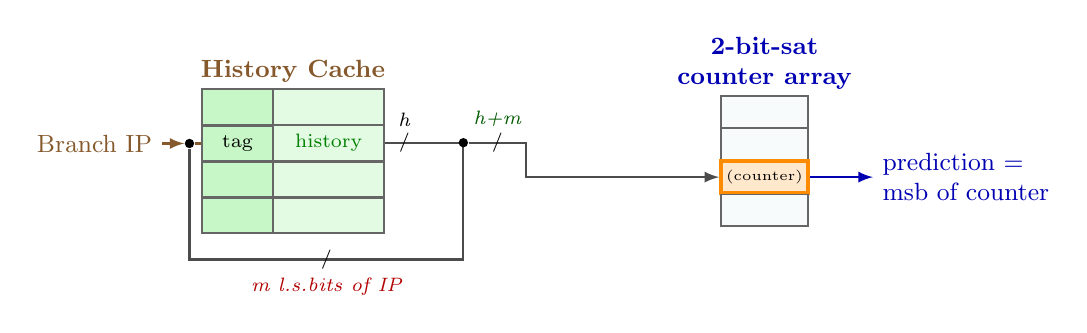
\begin{tikzpicture}[
    cache_cell/.style={draw=black!60, line width=0.6pt, minimum height=0.45cm, fill=lightgreen!30, inner sep=2pt, font=\scriptsize},
    counter_row/.style={draw=black!60, line width=0.6pt, minimum height=0.4cm, fill=lightblue!30, inner sep=1pt, font=\tiny},
    arrow/.style={-latex, thick, draw=black!70},
    data_connector/.style={circle, fill=black, inner sep=1.2pt}
]

    % History Cache using matrix of nodes (4 rows)
    \matrix[matrix of nodes,
        nodes={cache_cell},
        row sep=-\pgflinewidth,
        column sep=-\pgflinewidth,
        ampersand replacement=\&,
        label={[label distance=-5pt]above:{\small\bfseries\color{brown!70!black}History Cache}}
    ] (hist_cache) {
        |[minimum width=0.9cm, fill=lightgreen!50]| \& |[minimum width=1.4cm, fill=lightgreen!25]| \\
        |[minimum width=0.9cm, fill=lightgreen!50]| tag \& |[minimum width=1.4cm, fill=lightgreen!25]| \textcolor{mygreen}{history} \\
        |[minimum width=0.9cm, fill=lightgreen!50]| \& |[minimum width=1.4cm, fill=lightgreen!25]| \\
        |[minimum width=0.9cm, fill=lightgreen!50]| \& |[minimum width=1.4cm, fill=lightgreen!25]| \\
    };

    % Branch IP input - positioned relative to tag cell
    \node[anchor=east, left=0.5cm of hist_cache-2-1.west, font=\small, text=brown!70!black] (ip) {Branch IP};

    % Connector for branching off to m l.s.bits path
    \node[data_connector] (ip_conn) at ([xshift=-0.15cm]hist_cache-2-1.west) {};
    \draw[arrow, brown!70!black] (ip.east) -- (ip_conn);
    \draw[thick, brown!70!black] (ip_conn) -- (hist_cache-2-1.west);

    % Single shared counter array (vertical, 4 rows, highlight 3rd)
    \matrix[matrix of nodes,
        nodes={counter_row, minimum width=1.1cm},
        row sep=-\pgflinewidth,
        ampersand replacement=\&,
        right=4cm of hist_cache.east,
        anchor=west
    ] (counter_array) {
        |[fill=lightblue!10]| \\
        |[fill=lightblue!10]| \\
        |[draw=myorange, line width=1.5pt, fill=myorange!20, font=\tiny]| (counter) \\
        |[fill=lightblue!10]| \\
    };

    % Counter array title
    \node[above=-5pt of counter_array.north, font=\small\bfseries, text=blue!70!black, align=center] {2-bit-sat\\counter array};

    % Meeting point for h and m paths
    \coordinate (meet_point) at ([xshift=1cm]hist_cache-2-2.east);

    % Arrow from history going right with "h" label, then down to meet point
    \draw[thick, draw=black!70] (hist_cache-2-2.east) -- ++(0.5,0)
        node[midway, sloped, font=\scriptsize] {/}
        node[midway, above=2pt, font=\scriptsize\itshape] {h}
        -- (meet_point);

    % Route from connector around history cache bottom with "m l.s.bits of IP" label
    \draw[thick, draw=black!70] (ip_conn)
        |- ([yshift=-0.2cm]hist_cache.south -| ip_conn)
        -- ([yshift=-0.2cm]hist_cache.south -| meet_point)
            node[midway, sloped, font=\scriptsize] {/}
            node[midway, below=3pt, font=\scriptsize\itshape, text=red!70!black] {m l.s.bits of IP}
        -- (meet_point);

    % Combined h+m path to counter array
    \node[data_connector] at (meet_point) (combine_conn) {};
    \draw[arrow] (combine_conn) -- ++(0.8,0)
        node[midway, sloped, font=\scriptsize] {/}
        node[midway, above=2pt, font=\scriptsize\itshape, text=mygreen!70!black] {h+m}
        |- (counter_array-3-1.west);

    % Prediction output - right of highlighted cell for straight arrow
    \node[anchor=west, right=0.8cm of counter_array-3-1.east, font=\small, text=blue!70!black, align=left] (prediction) {prediction =\\msb of counter};

    % Arrow from counter to prediction (straight)
    \draw[arrow, blue!70!black] (counter_array-3-1.east) -- (prediction.west);

\end{tikzpicture}
\end{center}

\vspace{-0.2cm}

\begin{alertblock}{Local Predictor with Lselect Size}
\small
Size = \#BHRs $\times$ (tag\_size + history\_size) + 2 $\times$ $2^{\text{history\_size} + m}$
\end{alertblock}

\end{frame}

% Local Predictor: Lshare
\begin{frame}
\frametitle{Local Predictor: \textit{Lshare}}
\label{frame:lshare}

\begin{itemize}
    \item \textbf{\textit{Lshare} reduces inter-branch-interference} in the counter array
    \item Counter array index = history $\oplus$ $h$ l.s.bits of IP (XOR)
    \item Maps common patterns in different branches to different counters
\end{itemize}

\vspace{-0.1cm}

\begin{center}
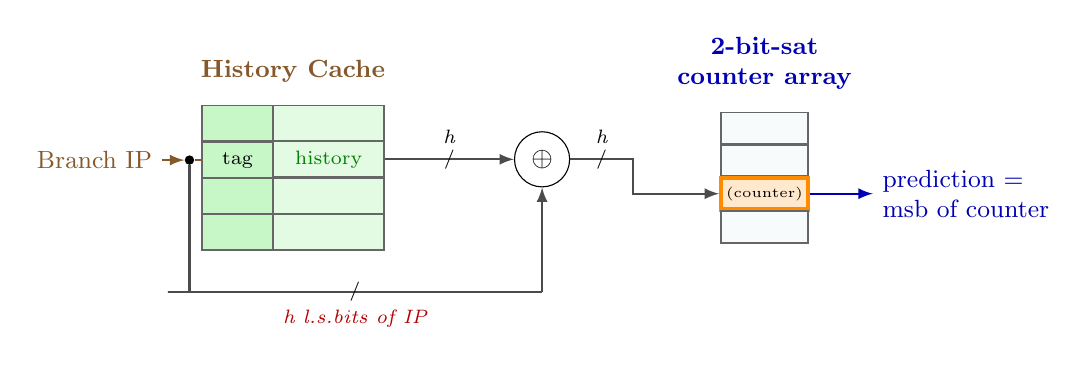
\begin{tikzpicture}[
    cache_cell/.style={draw=black!60, line width=0.6pt, minimum height=0.45cm, fill=lightgreen!30, inner sep=2pt, font=\scriptsize},
    counter_row/.style={draw=black!60, line width=0.6pt, minimum height=0.4cm, fill=lightblue!30, inner sep=1pt, font=\tiny},
    arrow/.style={-latex, thick, draw=black!70},
    data_connector/.style={circle, fill=black, inner sep=1.2pt}
]

    % History Cache using matrix of nodes (4 rows)
    \matrix[matrix of nodes,
        nodes={cache_cell},
        row sep=-\pgflinewidth,
        column sep=-\pgflinewidth,
        ampersand replacement=\&,
        label={[label distance=1pt]above:{\small\bfseries\color{brown!70!black}History Cache}}
    ] (hist_cache) {
        |[minimum width=0.9cm, fill=lightgreen!50]| \& |[minimum width=1.4cm, fill=lightgreen!25]| \\
        |[minimum width=0.9cm, fill=lightgreen!50]| tag \& |[minimum width=1.4cm, fill=lightgreen!25]| \textcolor{mygreen}{history} \\
        |[minimum width=0.9cm, fill=lightgreen!50]| \& |[minimum width=1.4cm, fill=lightgreen!25]| \\
        |[minimum width=0.9cm, fill=lightgreen!50]| \& |[minimum width=1.4cm, fill=lightgreen!25]| \\
    };

    % Branch IP input - positioned relative to tag cell
    \node[anchor=east, left=0.5cm of hist_cache-2-1.west, font=\small, text=brown!70!black] (ip) {Branch IP};

    % Connector for branching off to h l.s.bits path
    \node[data_connector] (ip_conn) at ([xshift=-0.15cm]hist_cache-2-1.west) {};
    \draw[arrow, brown!70!black] (ip.east) -- (ip_conn);
    \draw[thick, brown!70!black] (ip_conn) -- (hist_cache-2-1.west);

    % XOR gate
    \node[draw, circle, minimum size=0.7cm] (xor) at ([xshift=2cm]hist_cache-2-2.east) {$\oplus$};

    % Single shared counter array (vertical, 4 rows, highlight 3rd)
    \matrix[matrix of nodes,
        nodes={counter_row, minimum width=1.1cm},
        row sep=-\pgflinewidth,
        ampersand replacement=\&,
        right=4cm of hist_cache.east,
        anchor=west
    ] (counter_array) {
        |[fill=lightblue!10]| \\
        |[fill=lightblue!10]| \\
        |[draw=myorange, line width=1.5pt, fill=myorange!20, font=\tiny]| (counter) \\
        |[fill=lightblue!10]| \\
    };

    % Counter array title
    \node[above=1pt of counter_array.north, font=\small\bfseries, text=blue!70!black, align=center] {2-bit-sat\\counter array};

    % Arrow from history going right to XOR with "h" label
    \draw[arrow] (hist_cache-2-2.east) -- (xor.west)
        node[midway, sloped, font=\scriptsize] {/}
        node[midway, above=2pt, font=\scriptsize\itshape] {h};

    % Route from connector around history cache bottom with "h l.s.bits of IP" label
    \draw[thick, draw=black!70] (ip_conn)
        |- ([xshift=-0.3cm, yshift=-0.4cm]hist_cache.south west)
        -- ([yshift=-0.4cm]hist_cache.south -| xor)
            node[midway, sloped, font=\scriptsize] {/}
            node[midway, below=3pt, font=\scriptsize\itshape, text=red!70!black] {h l.s.bits of IP};
    \draw[arrow] ([yshift=-0.4cm]hist_cache.south -| xor) -- (xor.south);

    % XOR to counter array with "h" label
    \draw[arrow] (xor.east) -- ++(0.8,0)
        node[midway, sloped, font=\scriptsize] {/}
        node[midway, above=2pt, font=\scriptsize\itshape] {h}
        |- (counter_array-3-1.west);

    % Prediction output - right of highlighted cell for straight arrow
    \node[anchor=west, right=0.8cm of counter_array-3-1.east, font=\small, text=blue!70!black, align=left] (prediction) {prediction =\\msb of counter};

    % Arrow from counter to prediction (straight)
    \draw[arrow, blue!70!black] (counter_array-3-1.east) -- (prediction.west);

\end{tikzpicture}
\end{center}

\vspace{0.2cm}

\begin{alertblock}{Local Predictor with Lshare Size}
\small
Size = \#BHRs $\times$ (tag\_size + history\_size) + 2 $\times$ $2^{\text{history\_size}}$
\end{alertblock}

\end{frame}

\subsection{Global History Predictors}

\begin{frame}
\frametitle{Global Predictor}
\label{frame:global_predictor}

\begin{itemize}
    \item The behavior of some branches is \textbf{highly correlated}
\end{itemize}

\begin{center}
\begin{tcolorbox}[
    colback=lightblue!10,
    colframe=myblue,
    boxrule=1pt,
    arc=2mm,
    left=3mm, right=3mm, top=2mm, bottom=2mm,
    fontupper=\small\ttfamily,
    width=0.85\textwidth
]
if (x < 1) \{ ... \}  \textcolor{black!60}{// branch A}

if (x > 1) \{ ... \}  \textcolor{black!60}{// branch B: if A taken $\Rightarrow$ B not taken!}
\end{tcolorbox}
\end{center}

\begin{itemize}
    \item \textbf{Global History Register (GHR):} single history shared by all branches
\end{itemize}

\begin{center}
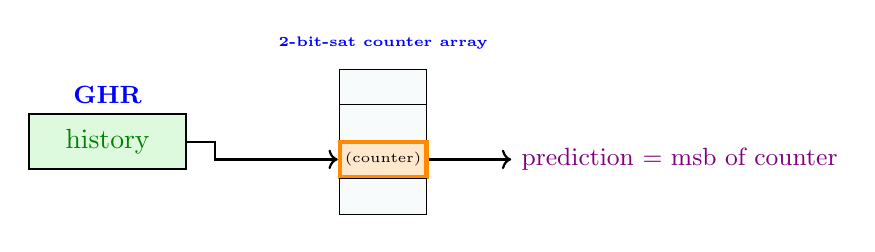
\begin{tikzpicture}[scale=0.7]
    % GHR
    \node[draw,thick,fill=lightgreen!30,minimum width=2cm,minimum height=0.7cm] (ghr) at (0,0) {\textcolor{mygreen}{history}};
    \node[anchor=south,font=\small\bfseries,myblue] at (ghr.north) {GHR};

    % Counter array as matrix of nodes
    \matrix[matrix of nodes,
            nodes={draw, minimum width=1.1cm, minimum height=0.45cm, anchor=center, fill=lightblue!10, inner sep=1pt},
            row sep=-\pgflinewidth, column sep=-\pgflinewidth,
            anchor=west] (counter_array) at (4,0) {
        |[fill=lightblue!10]| \\
        |[fill=lightblue!10]| \\
        |[draw=myorange, line width=1.5pt, fill=myorange!20, font=\tiny]| (counter) \\
        |[fill=lightblue!10]| \\
    };
    \node[anchor=south,font=\tiny\bfseries,myblue] at (counter_array.north) {2-bit-sat counter array};

    % Arrows
    \draw[->,thick] (ghr.east) -- ++(0.5,0) |- (counter_array-3-1.west);
    \draw[->,thick] (counter_array-3-1.east) -- ++(1.5,0)
        node[anchor=west,font=\small,mypurple] {prediction = msb of counter};
\end{tikzpicture}
\end{center}

\begin{itemize}
    \item History interference between non-correlated branches may hurt prediction
    \item With a single history, can afford a \textbf{long history}
    \begin{itemize}
        \item Predictor size: history\_size + 2$\times$$2^{\text{history\_size}}$
    \end{itemize}
\end{itemize}

\end{frame}

% Global Predictor: Gshare
\begin{frame}
\frametitle{Global Predictor: \textit{Gshare}}
\label{frame:gshare}

\begin{itemize}
    \item \textbf{Gshare:} combines global history with the branch IP using XOR
\end{itemize}

\vspace{0.3cm}

\begin{center}
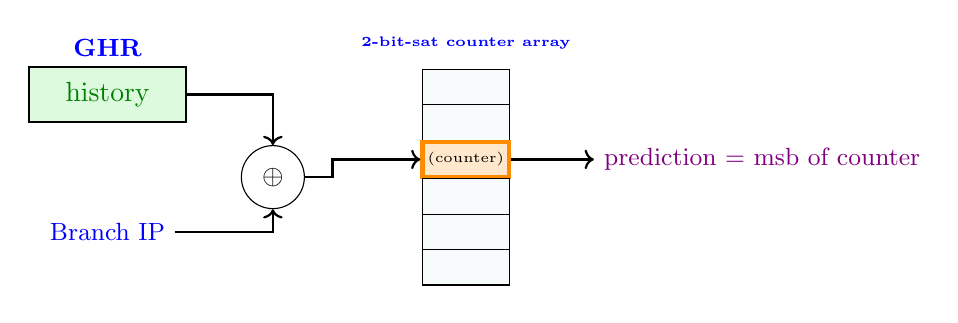
\begin{tikzpicture}[scale=0.7]
    % XOR
    \node[draw,circle,minimum size=0.8cm] (xor) at (3,0) {$\oplus$};

    % GHR (above and left of xor)
    \node[draw,thick,fill=lightgreen!30,minimum width=2cm,minimum height=0.7cm] (ghr) at (0,1.5) {\textcolor{mygreen}{history}};
    \node[anchor=south,font=\small\bfseries,myblue] at (ghr.north) {GHR};

    % Branch IP (below GHR, symmetric y-delta from xor)
    \node[font=\small,myblue] (branchip) at ([yshift=-1cm]ghr |- xor) {Branch IP};

    % Counter array as matrix of nodes
    \matrix[matrix of nodes,
            nodes={draw, minimum width=1.1cm, minimum height=0.45cm, anchor=center, fill=lightblue!10, inner sep=1pt},
            row sep=-\pgflinewidth, column sep=-\pgflinewidth,
            anchor=west] (counter_array) at (5.5,0) {
        |[fill=lightblue!10]| \\
        |[fill=lightblue!10]| \\
        |[draw=myorange, line width=1.5pt, fill=myorange!20, font=\tiny]| (counter) \\
        |[fill=lightblue!10]| \\
        |[fill=lightblue!10]| \\
        |[fill=lightblue!10]| \\
    };
    \node[anchor=south,font=\tiny\bfseries,myblue] at (counter_array.north) {2-bit-sat counter array};

    % Arrows
    \draw[->,thick] (ghr.east) -| (xor.north);
    \draw[->,thick] (branchip.east) -| (xor.south);
    \draw[->,thick] (xor.east) -- ++(0.5,0) |- (counter_array-3-1.west);
    \draw[->,thick] (counter_array-3-1.east) -- ++(1.5,0)
        node[anchor=west,font=\small,mypurple] {prediction = msb of counter};
\end{tikzpicture}
\end{center}

\vspace{0.3cm}

\begin{itemize}
    \item Counter index = GHR $\oplus$ Branch IP
    \begin{itemize}
        \item Learns: ``following this history, at this branch $\rightarrow$ taken/not-taken''
    \end{itemize}
    \item Turns out to be \textbf{extremely accurate} and space-efficient
\end{itemize}

\end{frame}

% Why Gshare Works So Well
\begin{frame}
\frametitle{Why \textit{Gshare} Works So Well}
\label{frame:why_gshare}

\begin{itemize}
    \item Updating a single history with all branches' outcomes might seem chaotic, but...
    \item The \textbf{number of active branches} at any moment is usually small
\end{itemize}

\vspace{0.3cm}

\textbf{Example 1:} A short loop with no \texttt{if} statements
\begin{itemize}
    \item Only one branch exists $\Rightarrow$ Gshare behaves like local history
\end{itemize}

\vspace{0.3cm}

\textbf{Example 2:} Two active branches A and B
\begin{itemize}
    \item GHR contains interleaved outcomes from both
    \item XOR with different IPs $\Rightarrow$ A and B update \textbf{different counters}
\end{itemize}

\end{frame}

% Chooser
\begin{frame}
\frametitle{Chooser}
\label{frame:chooser}

\begin{center}
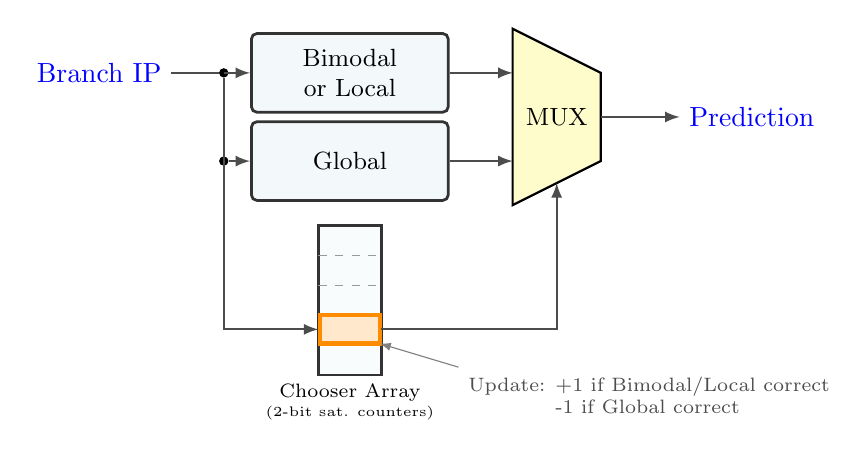
\begin{tikzpicture}[
    box/.style={draw=black!80, line width=1pt, minimum height=1cm, minimum width=2.5cm, fill=lightblue!15, rounded corners=2pt, font=\small},
    arrow/.style={-latex, thick, draw=black!70},
    data_connector/.style={circle, fill=black, inner sep=1.2pt}
]

    % MUX using circuitikz muxdemux
    \node[muxdemux, muxdemux def={Lh=4, Rh=2, NL=2, NB=1, w=2},
          external pins width=0, fill=yellow!20, anchor=lpin 2] (mux) {};

    % Bimodal or Local box
    \node[box, align=center, left=0.8cm of mux.lpin 1, anchor=east] (bimodal) {Bimodal\\or Local};

    % Branch IP input
    \node[font=\normalsize, text=myblue, left=1cm of bimodal.west] (branch_ip) {Branch IP};

    % Connector for Branch IP
    \node[data_connector, right=0.6cm of branch_ip.east] (conn) {};

    % Global box
    \node[box, left=0.8cm of mux.lpin 2] (global) {Global};

    % Chooser array - drawn with loop and dashed lines, closer to global
    \coordinate (array_start) at ([yshift=-0.3cm]global.south);

    % Draw array box outline - smaller
    \draw[draw=black!80, line width=1pt, fill=lightblue!8]
      ([xshift=-0.4cm]array_start) rectangle ++(0.8cm, -1.9cm)
      node[pos=0.5] (chooser_center) {};

    % Draw dashed lines to show array elements - aligned properly
    \foreach \i in {1,2,3,4} {
      \draw[dashed, black!40] ([xshift=-0.4cm, yshift=-\i*0.38cm]array_start) -- ++(0.8cm, 0);
    }

    % Highlight one element in the middle - aligned with dashed lines
    \draw[draw=myorange, line width=1.5pt, fill=myorange!20]
      ([xshift=-0.38cm, yshift=-1.14cm]array_start) rectangle ++(0.76cm, -0.36cm)
      coordinate[pos=1] (highlight_se);

    % Label for chooser array - BELOW the array
    \node[below=0.8cm of chooser_center.south, font=\scriptsize, text=black, align=center, anchor=north]
      {Chooser Array\\[-1pt]\tiny (2-bit sat. counters)};

    % Store chooser position for connections
    \coordinate (chooser_west) at ([xshift=-0.4cm, yshift=-1.32cm]array_start);
    \coordinate (chooser_east) at ([xshift=0.4cm, yshift=-1.32cm]array_start);

    % Label for MUX
    \node at (mux.center) [font=\small] {MUX};

    % Prediction output
    \node[right=1cm of mux.rpin 1, font=\normalsize, text=myblue] (prediction) {Prediction};

    % Arrows - Branch IP to all three components
    \draw[thick, draw=black!70] (branch_ip) -- (conn);
    \draw[arrow] (conn) |- (bimodal.west);
    \node[data_connector] (conn2) at (conn |- global.west) {};
    \draw[thick, draw=black!70] (conn) -- (conn2);
    \draw[arrow] (conn2) -- (global.west);
    \draw[arrow] (conn) |- (chooser_west);

    % Arrows - from predictors to MUX
    \draw[arrow] (bimodal.east) -- ++(0.3, 0) |- (mux.lpin 1);
    \draw[arrow] (global.east) -- ++(0.3, 0) |- (mux.lpin 2);

    % Arrow - Chooser to MUX control (bottom pin)
    \draw[arrow] (chooser_east) -| (mux.bpin 1);

    % Arrow - MUX to Prediction
    \draw[arrow] (mux.rpin 1) -- (prediction);

    % Add update explanation right below the highlighted box
    \node[anchor=north west, font=\scriptsize, text=black!70, align=left] (update_text)
      at ([xshift=1cm, yshift=-0.3cm]highlight_se) {
      Update: +1 if Bimodal/Local correct\\
      \phantom{Update: }-1 if Global correct
    };

    % Arrow from text to highlighted box
    \draw[-latex, draw=black!50, thin] (update_text.north west) -- (highlight_se);

\end{tikzpicture}
\end{center}

\vspace{-0.1cm}

\begin{itemize}
    \item \textbf{Chooser selects between two predictors}
    \begin{itemize}
        \item Array of 2-bit saturating counters indexed by \textcolor{myblue}{Branch IP}
        \item Each counter tracks which predictor performs better for that branch
        \item MUX selects the prediction from the better predictor
    \end{itemize}
\end{itemize}

\vspace{0.2cm}

\begin{itemize}
    \item \textbf{Counter update policy (at execution):}
    \begin{itemize}
        \item \textcolor{mygreen}{Increment}: if Bimodal/Local correct \textit{and} Global wrong
        \item \textcolor{red}{Decrement}: if Global correct \textit{and} Bimodal/Local wrong
        \item No change if both correct or both wrong
    \end{itemize}
\end{itemize}

\end{frame}

\section{Indirect Branch Target Prediction}

\begin{frame}
\frametitle{Indirect Branch Target Prediction}
\label{frame:indirect_target_1}

\begin{itemize}
    \item \textbf{Indirect branches:} target given in a register
    \begin{itemize}
        \item Can have many targets (e.g., switch/case statements)
        \item Resolved at execution $\Rightarrow$ high misprediction penalty
        \item Common in object-oriented code (C++, Java)
    \end{itemize}
    \item \textbf{History-based prediction:} uses the same GHR as conditional branches
\end{itemize}

\vspace{0.3cm}

\begin{center}
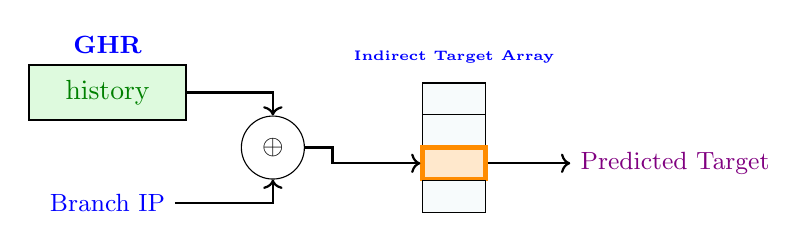
\begin{tikzpicture}[scale=0.7]
    % XOR
    \node[draw,circle,minimum size=0.8cm] (xor) at (3,0) {$\oplus$};

    % GHR (above and left of xor)
    \node[draw,thick,fill=lightgreen!30,minimum width=2cm,minimum height=0.7cm] (ghr) at ([xshift=-3cm,yshift=1cm]xor) {\textcolor{mygreen}{history}};
    \node[anchor=south,font=\small\bfseries,myblue] at (ghr.north) {GHR};

    % Branch IP (below GHR, symmetric y-delta from xor)
    \node[font=\small,myblue] (branchip) at ([yshift=-1cm]ghr |- xor) {Branch IP};

    % Indirect Target Array as matrix of nodes
    \matrix[matrix of nodes,
            nodes={draw, minimum width=0.8cm, minimum height=0.4cm, anchor=center, fill=lightblue!10, inner sep=1pt},
            row sep=-\pgflinewidth, column sep=-\pgflinewidth,
            anchor=west] (ita) at (5.5,0) {
        |[fill=lightblue!10]| \\
        |[fill=lightblue!10]| \\
        |[draw=myorange, line width=1.5pt, fill=myorange!20]| \\
        |[fill=lightblue!10]| \\
    };
    \node[anchor=south,font=\tiny\bfseries,myblue] at (ita.north) {Indirect Target Array};

    % Arrows
    \draw[->,thick] (ghr.east) -| (xor.north);
    \draw[->,thick] (branchip.east) -| (xor.south);
    \draw[->,thick] (xor.east) -- ++(0.5,0) |- (ita-3-1.west);
    \draw[->,thick] (ita-3-1.east) -- ++(1.5,0)
        node[anchor=west,font=\small,mypurple] {Predicted Target};
\end{tikzpicture}
\end{center}

\begin{itemize}
    \item Each jump uses multiple entries\\
          $\Rightarrow$ more expensive than TA\\
          $\Rightarrow$ use only for multi-target jumps
\end{itemize}

\end{frame}

\begin{frame}
\frametitle{Indirect Target Array (iTA) Allocation}
\label{frame:indirect_target_2}

\begin{itemize}
    \item \textbf{Initial allocation:} indirect branch stored only in Target Array (TA)
    \begin{itemize}
        \item Many indirect branches have only one target
    \end{itemize}
    \item \textbf{On TA misprediction:} allocate iTA entry indexed by IP $\oplus$ GHR
    \item \textbf{Use iTA prediction} when TA indicates indirect jump and iTA hits
\end{itemize}

\vspace{0.1cm}

\begin{center}
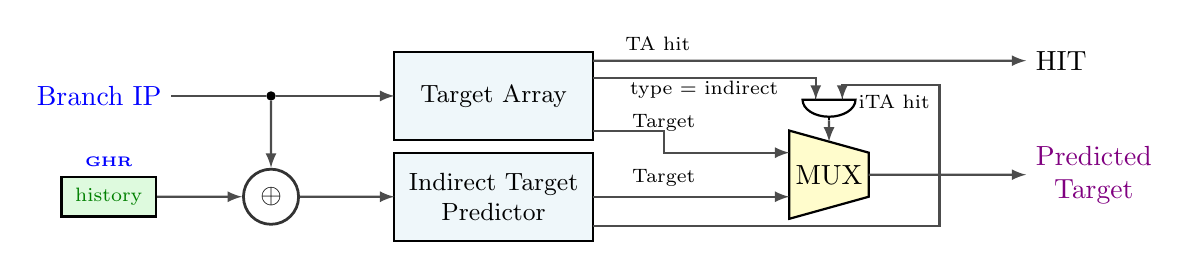
\begin{tikzpicture}[scale=0.9,
    arrow/.style={-latex, thick, draw=black!70},
    signal/.style={font=\scriptsize},
    data_connector/.style={circle, fill=black, inner sep=1.2pt}
]

    % Branch IP input (anchor point)
    \node[font=\normalsize, text=myblue] (branch_ip) at (0,0) {Branch IP};

    % Connector for Branch IP
    \node[data_connector, right=1.2cm of branch_ip] (conn_ip) {};

    % Target Array as muxdemux - wider and shorter (Lh=Rh, slightly wider)
    \node[muxdemux, muxdemux def={Lh=2, Rh=2, NL=1, NR=5, w=4.5},
          external pins width=0, fill=lightblue!20, anchor=lpin 1, right=1.5cm of conn_ip, align=center,
          font=\small] (ta) {Target Array};

    % Main MUX for output selection - now with top pin, positioned lower
    \node[muxdemux, muxdemux def={Lh=2, Rh=1, NL=2, NB=0, NR=1, w=1.8, NT=1},
          external pins width=0, fill=yellow!20, xshift=3cm, yshift=-1cm] (mux) at (ta.east) {MUX};

    % Indirect Target Predictor - wider and shorter, positioned using |- relative to TA and MUX
    \node[muxdemux, muxdemux def={Lh=2, Rh=2, NL=1, NR=3, w=4.5},
          external pins width=0, fill=lightblue!20, anchor=rpin 2, align=center, font=\small] (itp) at (ta.east |- mux.lpin 2) {Indirect Target\\Predictor};

    % XOR gate positioned using |- with conn_ip x-axis and itp y-axis
    \node[circle, draw=black!80, line width=1pt, minimum size=0.7cm, fill=white] (xor) at (conn_ip |- itp.lpin 1) {$\oplus$};

    % GHR - positioned using |- with branch_ip x-axis and xor y-axis
    \node[draw, thick, fill=lightgreen!30, minimum width=1.2cm, minimum height=0.5cm,
          anchor=east, font=\scriptsize] (ghr) at ([xshift=-2mm]branch_ip.east |- xor) {\textcolor{mygreen}{history}};
    \node[anchor=south, font=\tiny\bfseries, myblue] at (ghr.north) {GHR};

    % AND gate rotated 90 degrees - smaller, anchored at output pin above MUX top pin
    \node[and port, rotate=-90, xscale=0.2, yscale=0.6, anchor=out, external pins width=0,
          logic gate input sep=0pt] at ([yshift=3mm]mux.tpin 1) (and_gate) {};

    % Output
    \node[font=\normalsize, text=mypurple, right=2cm of mux.rpin 1, align=center] (pred_target) {Predicted\\Target};

    % HIT output from TA - positioned at intersection of ta.rpin 1 y-coordinate and pred_target.west x-coordinate
    \coordinate (hit_pos) at (pred_target.west |- ta.rpin 1);
    \node[font=\normalsize, text=black, anchor=west] (hit_out) at (hit_pos) {HIT};

    % Draw connections
    % Branch IP to connector
    \draw[thick, draw=black!70] (branch_ip) -- (conn_ip);

    % Branch IP to Target Array
    \draw[arrow] (conn_ip) -- (ta.lpin 1);

    % Branch IP to XOR gate - goes to xor.north
    \draw[arrow] (conn_ip) -- (xor.north);

    % GHR to XOR gate
    \draw[arrow] (ghr.east) -- (xor.west);

    % XOR to Indirect Target Predictor
    \draw[arrow] (xor.east) -- (itp.lpin 1);

    % Target Array outputs (3 rpins: rpin 1 = TA hit, rpin 2 = type=indirect, rpin 3 = target)
    % rpin 1: TA hit to HIT
    \draw[arrow] (ta.rpin 1) -- (hit_out.west) node[signal, pos=0.15, above] {TA hit};

    % rpin 2: type = indirect to AND gate input 1
    \draw[arrow] (ta.rpin 2) -| (and_gate.bin 2) node[signal, pos=0.25, below, yshift=1mm] {type = indirect};

    % rpin 3: Target to MUX lpin 1
    \draw[arrow] (ta.rpin 5) -- ++(1,0) coordinate (ta_target_corner) |- (mux.lpin 1) node[signal, pos=0.25, above] {Target};

    % Indirect Target Predictor outputs (3 rpins: rpin 1 = Target, rpin 2 = iTA hit, rpin 3 unused)
    % rpin 1: Target to MUX lpin 2
    \draw[arrow] (itp.rpin 2) -- ++(1,0) coordinate (itp_target_corner) |- (mux.lpin 2) node[signal, pos=0.25, above] {Target};

    % rpin 2: iTA hit to AND gate input 2 with complex routing
    \draw[arrow] (itp.rpin 3) -| ([xshift=1cm]mux.east) |- ([xshift=1cm,yshift=5mm]and_gate.east) -| (and_gate.bin 1) node[signal, pos=0.05, below] {iTA hit};

    % AND gate output to MUX top pin
    \draw[arrow] (and_gate.out) -- (mux.tpin 1);

    % MUX to Predicted Target
    \draw[arrow] (mux.rpin 1) -- (pred_target.west);

\end{tikzpicture}
\end{center}

\end{frame}

% Return Stack Buffer
\begin{frame}
\frametitle{Return Stack Buffer}
\label{frame:rsb}

\begin{itemize}
    \item \textbf{A return instruction is a special case of an indirect branch}
    \begin{itemize}
        \item Each times it jumps to a different target
        \item The target is determined by the location of the corresponding Call instruction
    \end{itemize}
\end{itemize}

\vspace{0.3cm}

\begin{itemize}
    \item \textbf{Maintain a small stack of targets at fetch time}
    \begin{itemize}
        \item When the Target Array predicts a Call
        \begin{itemize}
            \item Push the address of the instruction which follows the Call into the stack (this is the predicted Return address)
        \end{itemize}
        \item When the Target Array predicts a Return
        \begin{itemize}
            \item Pop a target from the stack and use it as the Return address
        \end{itemize}
    \end{itemize}
\end{itemize}

\end{frame}

% RSB Operation Illustration
\begin{frame}
\frametitle{Return Stack Buffer Operation}
\label{frame:rsb_operation}

% Define colors for each function
\definecolor{mainfill}{RGB}{200,230,200}
\definecolor{func1fill}{RGB}{255,220,220}
\definecolor{func2fill}{RGB}{220,220,255}

\begin{center}
\begin{tikzpicture}[scale=0.85,
    remember picture,
    codebox/.style={draw=black!80, line width=1pt, minimum width=3cm, minimum height=1.2cm, font=\footnotesize\ttfamily, text width=2.8cm, align=left},
    arrow/.style={-latex, thick, draw=black!70},
    label/.style={font=\scriptsize, text=black}
]

    % Code boxes on the left
    \node[codebox, fill=mainfill] (main) at (0,0) {main:\\~~...\\~~call~~func1\\~~...\\~~ret};
    \node[codebox, fill=func1fill, below=0.5cm of main] (func1) {func1:\\~~...\\~~call~~func2\\~~...\\~~ret};
    \node[codebox, fill=func2fill, below=0.5cm of func1] (func2) {func2:\\~~...\\~~ret};

    % Invisible marker nodes for arrows
    \coordinate (call1) at ([xshift=1.3cm, yshift=-0.3cm]main.west);
    \coordinate (call2) at ([xshift=1.3cm, yshift=-0.3cm]func1.west);
    \coordinate (ret2) at ([xshift=1.3cm, yshift=-0.65cm]func2.west);

    % Stack on the right using matrix
    \node[label, right=5cm of main.north east, anchor=south] (stack_label) {Stack};

    \matrix[matrix of nodes, below=-0.05cm of stack_label, anchor=north,
            nodes={draw=black!80, line width=0.5pt, minimum width=2.5cm, minimum height=0.5cm,
                   font=\scriptsize, anchor=center},
            row sep=0pt, column sep=0pt] (stack_matrix) {
        |[fill=func2fill]| ... \\
        |[fill=func2fill]| retaddr2 \\
        |[fill=func2fill]| Arguments \\
        |[fill=func1fill]| ... \\
        |[fill=func1fill]| retaddr1 \\
        |[fill=func1fill]| Arguments \\
        |[fill=mainfill]| ... \\
    };

    % Frame braces and labels
    \draw[thick, decoration={brace, amplitude=5pt}, decorate]
        ([xshift=0.25cm]stack_matrix-1-1.north east) -- ([xshift=0.25cm]stack_matrix-3-1.south east)
        node[midway, right=0.15cm, font=\tiny, align=left] {Frame\\of func2};

    \draw[thick, decoration={brace, amplitude=5pt}, decorate]
        ([xshift=0.25cm]stack_matrix-4-1.north east) -- ([xshift=0.25cm]stack_matrix-6-1.south east)
        node[midway, right=0.15cm, font=\tiny, align=left] {Frame\\of func1};

    % RSB below the stack using matrix
    \node[label, below=0.5cm of stack_matrix, anchor=north] (rsb_label) {RSB};

    \matrix[matrix of nodes, below=-0.05cm of rsb_label, anchor=north,
            nodes={draw=black!80, line width=0.5pt, minimum width=2.5cm, minimum height=0.5cm,
                   font=\scriptsize, anchor=center},
            row sep=0pt, column sep=0pt] (rsb_matrix) {
        |[fill=func2fill]| retaddr2 \\
        |[fill=func1fill]| retaddr1 \\
        |[fill=green!15]| ... \\
    };

    % Arrows showing the flow
    % Arrow 1: Load from stack - from ret instruction in func2
    \draw[arrow] (ret2) -- ++(3,0) |- (stack_matrix-2-1.west)
        node[near end, above, align=center, font=\scriptsize, text=black] {Load\\from\\stack};

    % Arrow 2: Consult for prediction - from ret instruction in func2
    \draw[arrow] (ret2) -- ++(3,0) |- (rsb_matrix-1-1.west)
        node[near end, above, align=center, font=\scriptsize, text=black] {Consult\\for prediction};

    % Labels for return addresses
    \node[font=\scriptsize, text=black, fill=func1fill, inner sep=2pt, anchor=east] at ([xshift=-0.2cm]call1 -| main.west) {retaddr1};
    \node[font=\scriptsize, text=black, fill=func2fill, inner sep=2pt, anchor=east] at ([xshift=-0.2cm]call2 -| main.west) {retaddr2};

\end{tikzpicture}
\end{center}

\vspace{0.3cm}

\begin{itemize}
    \item \textbf{At return: processor loads from stack (slow) while consulting RSB for prediction (fast)}
\end{itemize}

\end{frame}

\section{Real-World Implementations}

\begin{frame}
\frametitle{Intel 486, Pentium\textsuperscript{\textregistered}, Pentium\textsuperscript{\textregistered} II}
\label{frame:intel_predictors}

\begin{itemize}
    \item \textbf{486} \hspace{1cm} Statically predict Not Taken
    \item \textbf{Pentium\textsuperscript{\textregistered}} \hspace{1cm} 2-bit saturating counters
    \item \textbf{Pentium\textsuperscript{\textregistered} II}
    \begin{itemize}
        \item 2-level, local histories, per-set counters
        \item 4-way set associative: 512 entries in 128 sets
    \end{itemize}
\end{itemize}

\vspace{0.3cm}

\begin{center}
% TODO: Add Pentium II predictor diagram
\textcolor{red}{[PLACEHOLDER: Pentium II predictor structure diagram]}
\end{center}

\end{frame}

% Alpha 264 - LG Chooser
\begin{frame}
\frametitle{Alpha 21264: Local-Global Chooser}
\label{frame:alpha_264}

\begin{center}
% TODO: Add Alpha 264 predictor diagram
\textcolor{red}{[PLACEHOLDER: Alpha 264 LG Chooser architecture diagram]}
\end{center}

\vspace{0.3cm}

\begin{itemize}
    \item New entry on the Local stage is allocated on a global stage mis-prediction
    \item Chooser state-machines: 2 bit each:
    \begin{itemize}
        \item one bit saves last time global correct/wrong
        \item and the other bit saves for the local correct/wrong
    \end{itemize}
    \item Chooses Local only if local was correct and global was wrong
\end{itemize}

\end{frame}


\end{document}